%% 
%% Copyright 2007-2024 Elsevier Ltd
%% 
%% This file is part of the 'Elsarticle Bundle'.
%% ---------------------------------------------
%% 
%% It may be distributed under the conditions of the LaTeX Project Public
%% License, either version 1.3 of this license or (at your option) any
%% later version.  The latest version of this license is in
%%    http://www.latex-project.org/lppl.txt
%% and version 1.3 or later is part of all distributions of LaTeX
%% version 1999/12/01 or later.
%% 
%% The list of all files belonging to the 'Elsarticle Bundle' is
%% given in the file `manifest.txt'.
%% 
%% Template article for Elsevier's document class `elsarticle'
%% with numbered style bibliographic references
%% SP 2008/03/01
%% $Id: elsarticle-template-num.tex 249 2024-04-06 10:51:24Z rishi $
%%
\documentclass[final,1p,times]{elsarticle}
% Allow inclusion of PDF 1.7 figures without version mismatch warnings
\pdfminorversion=7

%% Use the option review to obtain double line spacing
%% \documentclass[authoryear,preprint,review,12pt]{elsarticle}

%% Use the options 1p,twocolumn; 3p; 3p,twocolumn; 5p; or 5p,twocolumn
%% for a journal layout:
%% \documentclass[final,1p,times]{elsarticle}
%% \documentclass[final,1p,times,twocolumn]{elsarticle}
%% \documentclass[final,3p,times]{elsarticle}
%% \documentclass[final,3p,times,twocolumn]{elsarticle}
%% \documentclass[final,5p,times]{elsarticle}
%% \documentclass[final,5p,times,twocolumn]{elsarticle}

%% For including figures, graphicx.sty has been loaded in
%% elsarticle.cls. If you prefer to use the old commands
%% please give \usepackage{epsfig}

%% The amssymb package provides various useful mathematical symbols
% \usepackage{cite}
\usepackage{amsmath,amssymb,amsfonts}
% \usepackage{algorithmic}
\usepackage[ruled,vlined]{algorithm2e}
\usepackage{graphicx}
% \usepackage{algorithm,algorithmic}
\usepackage[psdextra]{hyperref}
\usepackage{xurl}
% \usepackage[numbers,sort&compress]{natbib}
\usepackage[caption=false,font=footnotesize,labelfont=sf,textfont=sf]{subfig}
\usepackage{array}
\usepackage{balance}
\usepackage{placeins}
\setcounter{topnumber}{3}
\setcounter{bottomnumber}{2}
\setcounter{totalnumber}{4}
\renewcommand{\topfraction}{0.9}
\renewcommand{\bottomfraction}{0.8}
\renewcommand{\textfraction}{0.07}
\renewcommand{\floatpagefraction}{0.8}
\setlength{\emergencystretch}{2em}
% \usepackage{enumitem}       % For customizable lists (conflicts with IEEEtran)
\usepackage{booktabs}       % For professional tables with \toprule, \midrule, etc.
\usepackage{multirow}       % For table cells spanning multiple rows
\usepackage{makecell}       % For better table cell formatting
\usepackage{tikz}           % For flowcharts or block diagrams
\usetikzlibrary{shapes,arrows.meta,positioning,calc,shadows,backgrounds,decorations.pathreplacing,fit,petri,arrows}

% Hyperref setup: colored citations and links, enable Unicode, and safer PDF string handling
\hypersetup{
  colorlinks=true,
  linkcolor=blue,
  citecolor=blue,
  urlcolor=blue,
  hypertexnames=false,
  unicode=true,
  pdfencoding=auto,
  pdftitle={MSAGAT-Net: Multi-Scale Temporal Adaptive Graph Attention for Efficient Spatiotemporal Epidemic Forecasting},
  pdfauthor={Michael Ajao-olarinoye, Vasile Palade, Fei He, Petra A. Wark, Seyed Mousavi, Zindoga Mukandavire}
}
% Disable/neutralize commands that can appear in PDF strings (titles, bookmarks)
\makeatletter
\pdfstringdefDisableCommands{%
  \let\thanks\@gobble%
  \let\footnote\@gobble%
  \let\cortext\@gobble%
  \let\cnotenum\@gobble%
}
\makeatother
\usepackage{textcomp}
\usepackage{silence}
%% \usepackage{amsthm}

%% The lineno packages adds line numbers. Start line numbering with
%% \begin{linenumbers}, end it with \end{linenumbers}. Or switch it on
%% for the whole article with \linenumbers.
%% \usepackage{lineno}

\journal{Artificial Intelligence in Medicine}

\begin{document}

\begin{frontmatter}

%% Title, authors and addresses

%% use the tnoteref command within \title for footnotes;
%% use the tnotetext command for theassociated footnote;
%% use the fnref command within \author or \affiliation for footnotes;
%% use the fntext command for theassociated footnote;
%% use the corref command within \author for corresponding author footnotes;
%% use the cortext command for theassociated footnote;
%% use the ead command for the email address,
%% and the form \ead[url] for the home page:
%% \title{Title\tnoteref{label1}}
%% \tnotetext[label1]{}
%% \author{Name\corref{cor1}\fnref{label2}}
%% \ead{email address}
%% \ead[url]{home page}
%% \fntext[label2]{}
%% \cortext[cor1]{}
%% \affiliation{organization={},
%%             addressline={},
%%             city={},
%%             postcode={},
%%             state={},
%%             country={}}
%% \fntext[label3]{}

% \title{MSAGAT-Net: An Efficient Multi-Scale Temporal Graph Attention Network for Spatiotemporal Epidemic Forecasting}

\title{MSAGAT-Net: Multi-Scale Temporal Adaptive Graph Attention for Efficient Spatiotemporal Epidemic Forecasting}

%% use optional labels to link authors explicitly to addresses:
%% \author[label1,label2]{}
%% \affiliation[label1]{organization={},
%%             addressline={},
%%             city={},
%%             postcode={},
%%             state={},
%%             country={}}
%%
%% \affiliation[label2]{organization={},
%%             addressline={},
%%             city={},
%%             postcode={},
%%             state={},
%%             country={}}

% Authors and affiliations
% --- Authors ---
% \author[inst1]{Michael Ajao-olarinoye\corref{cor1}}
% \ead{olarinoyem@coventry.ac.uk}

% \author[inst1]{Vasile Palade}
% \author[inst1]{Fei He}
% \author[inst2]{Petra A.~Wark}
% \author[inst1]{Seyed Mousavi}
% \author[inst3]{Zindoga Mukandavire}

% --- Notes & correspondence ---
% \cortext[cor1]{Corresponding author.}
% \fntext[fn1]{These authors contributed equally to this work.}

% % --- Affiliations ---
% \affiliation[inst1]{%
%   organization={Centre for Computational Science and Mathematical Modelling, Coventry University},
%   city={Coventry},
%   country={United Kingdom}
% }

% \affiliation[inst2]{%
%   organization={Research Methods and Evaluation Unit, Research Centre for Healthcare and Communities, Coventry University},
%   city={Coventry},
%   country={United Kingdom}
% }

% \affiliation[inst3]{%
%   organization={Institute of Applied Research and Technology, Emirates Aviation University},
%   city={Dubai},
%   country={United Arab Emirates}
% }
\begin{abstract}
Accurate spatiotemporal epidemic forecasting is vital for preparedness and resource planning, yet many graph neural network approaches rely on predefined adjacency matrices, struggle to control how structural priors affect attention across varying graph densities, and become unstable at longer forecast horizons. We propose MSAGAT-Net, a multi-scale adaptive graph attention network that learns spatial dependencies directly from data while allowing optional adjacency priors. MSAGAT-Net introduces a self-attenuating additive structural bias by augmenting attention logits with a learnable low-rank graph bias and an optional adjacency prior before softmax. This design attenuates the prior’s influence on dense, near-uniform graphs via softmax shift-invariance, reducing the need for hand-tuned thresholds. The architecture further features an adaptive multi-hop spatial diffusion module whose depth scales with graph size to reduce oversmoothing, depthwise separable temporal feature extraction, and progressive prediction refinement for stable multi-horizon forecasts. Evaluated on diverse datasets spanning influenza, COVID-19, and ICU bed occupancy, MSAGAT-Net consistently outperforms strong baselines, achieving up to 23.5\% RMSE reduction on LTLA-COVID forecasting and 22.2\% on NHS-ICUBeds forecasting. Ablation results reveal horizon-dependent architectural importance, with adaptive spatial attention being universally essential while spatial refinement mechanisms grow increasingly critical as forecast difficulty increases.
\end{abstract}

% \begin{highlights}
% \item Self-attenuating graph attention adapts structural prior influence to graph density
% \item Adjacency-free spatial learning operates without predefined graph structures
% \item Adaptive multi-hop convolutions scale diffusion depth to graph size
% \item Up to 23.5\% RMSE reduction on 372-region COVID-19 forecasting
% \item Ablation across three graph scales reveals horizon-dependent component importance
% \end{highlights}

% Keywords (note: \begin{keywords} plural for CAS template)
% \begin{keywords}
% Graph neural networks \sep self-attenuating attention \sep adaptive graph learning \sep epidemic forecasting \sep spatiotemporal forecasting \sep multi-scale modelling
% \end{keywords}

\begin{keyword}
  Graph attention networks \sep adaptive graph learning \sep epidemic forecasting \sep spatiotemporal forecasting \sep multi-scale \sep public health surveillance
\end{keyword}

\end{frontmatter}

\section{Introduction}
\label{sec:introduction}

Accurate and timely epidemiological forecasting supports effective public health preparedness, enabling decision-makers to allocate clinical resources, plan interventions, and communicate risk before outbreaks escalate \cite{DEANGELIS201583, Brooks2018Nonmechanistic}. The COVID-19 pandemic underscored how rapidly disease dynamics can evolve across hundreds or thousands of interconnected regions \cite{ajao2023deep, da2021covid, giuliani2020modelling, verma2022temporal, ma2024reporting}, demanding computational methods that jointly model spatial propagation between regions and temporal patterns ranging from daily reporting fluctuations to seasonal waves \cite{Panja2022Epicasting, Stone2007Seasonal}. Traditional compartmental models such as SIR and SEIR provide valuable mechanistic insight but struggle with the heterogeneity and computational complexity required for real-time surveillance at this scale \cite{heltberg2022spatial, s25082507, DEANGELIS201583}.

Deep learning methods, first demonstrated in traffic forecasting \cite{li2017diffusion, zhang2021graph} and environmental monitoring \cite{wu2018deep, lai2018modeling}, have since advanced epidemic prediction through recurrent, convolutional, and graph neural network (GNN) architectures \cite{ajao2023deep, zhiweidingBiologyInformedRecurrentNeural2023, Ahmadini2025, Kamalov2022ReviewDL, wang2019defsi}. Among these, GNNs are particularly well suited to epidemic forecasting because they can learn complex spatiotemporal dependencies directly from data, outperforming traditional models in capturing regional heterogeneity and dynamic transmission mechanisms \cite{kimForecastingEpidemicSpread2025, lijingwangCausalGNNCausalBasedGraph2022, gao2021stan}. Graph attention networks \cite{velickovic2017graph} further improve spatial modelling by adaptively weighting inter-regional influence rather than relying on fixed graph convolution kernels.

Despite these advances, current GNN-based epidemic forecasting approaches face three fundamental limitations. First, existing graph attention mechanisms do not provide a principled way to regulate how much a structural prior, such as an adjacency matrix encoding geographic proximity, influences the learnt attention weights \cite{velickovic2017graph}. As a result, performance varies unpredictably across graphs of different density and size: the same attention design may overfit to structure on dense graphs while underutilising it on sparse ones. Second, state-of-the-art epidemic GNN such as EpiGNN \cite{xie2022epignn}, Cola-GNN \cite{dengColaGNNCrosslocationAttention2020a}, and DCRNN \cite{li2017diffusion} require adjacency matrices constructed from geographic proximity or mobility data. These matrices may not reflect true transmission pathways and presuppose domain expertise or external data sources that are often unavailable in practice, particularly during emerging outbreaks. Third, existing methods employ fixed architectural choices for spatial aggregation, such as a constant number of message-passing hops, which do not adapt to diverse graph sizes and disease dynamics. On small graphs this causes oversmoothing \cite{li2018deeper}, while on large graphs it limits receptive field coverage. Adding to this rigidity, the accumulation of errors across extended forecast horizons degrades the long-range predictions essential for public health planning \cite{Brooks2018Nonmechanistic}.

To address these limitations, we propose MSAGAT-Net (Multi-Scale Adaptive Graph Attention Network), an architecture designed to generalise across diverse graph topologies encountered in epidemic surveillance (7 to 372 regions in our experiments) without per-dataset tuning. MSAGAT-Net learns spatial relationships directly from data through a three-component additive attention mechanism whose structural prior influence self-attenuates with graph density, combined with graph-size-adaptive spatial aggregation that prevents oversmoothing and progressive prediction refinement for stable multi-horizon forecasts. Our key contributions are as follows:
 
\begin{enumerate}
  \item A three-component additive graph attention mechanism (EAGAM) that combines content-based attention scores with a learnable low-rank graph bias and an optional adjacency prior before softmax normalisation. The individual ingredients build on established ideas---additive structural bias in attention \cite{ying2021transformers, press2022train} and adaptive graph learning \cite{wu2020connecting, bai2020adaptive}---but, to the best of our knowledge, no existing epidemic forecasting model combines a learned graph bias with an optional adjacency prior in a single additive formulation; Section~\ref{sec:related_work} positions this design against both the epidemic and the general graph learning literature. Unlike existing epidemic GNNs that either ignore graph structure (content-only) or require it as mandatory input, EAGAM learns spatial relationships from data while allowing optional structural guidance whose influence self-attenuates with graph density.

  \item A graph-size-adaptive multi-hop spatial refinement module (MSSFM) that, unlike fixed-depth approaches used in existing epidemic GNNs, automatically adjusts diffusion depth to graph size and fuses multi-scale aggregations with locality-biased learnable weights, preventing oversmoothing on small graphs while preserving broader spatial context on larger ones.

  \item A systematic evaluation on six diverse epidemic datasets, with graph sizes ranging from 7 to 372 regions, demonstrating RMSE improvements of up to 23.5\% over the strongest baselines. To our knowledge, this is the first cross-scale ablation study in epidemic GNN literature, revealing that component importance is both horizon- and scale-dependent: adaptive spatial attention is essential on medium-to-large graphs, while progressive prediction refinement becomes increasingly critical at longer forecast horizons.
\end{enumerate}

The remainder of this paper is organised as follows. Section~\ref{sec:related_work} reviews related work. Section~\ref{sec:methodology} presents the formulation of the problem and the proposed architecture. Section~\ref{sec:experiments} describes the experimental setup. Section~\ref{sec:results} reports results and ablation studies. Section~\ref{sec:conclusion} concludes with limitations and future directions.

% ---------- SECTION II: LITERATURE REVIEW ----------
\section{Related Work}
\label{sec:related_work} 

Epidemic forecasting has evolved from classical compartmental models to neural network architectures that capture spatial coupling and temporal heterogeneity. This section reviews (i) spatiotemporal graph learning for epidemics, including attention-based, hybrid physics-informed, and transformer-based models that learn dynamic cross-regional influence, and (ii) multi-scale temporal modelling and multi-horizon forecasting strategies. We position MSAGAT-Net within this landscape by highlighting the lack of adaptive structural bias control in existing graph attention mechanisms, the rigidity of fixed architectural choices, and the need for stable long-range forecasts.

% \subsection{Graph Neural Networks for Spatiotemporal Epidemic Modelling}

\subsection{Spatiotemporal Epidemic Modelling}
The application of graph neural networks to epidemic forecasting has emerged as a dominant paradigm, fundamentally addressing limitations of traditional compartmental models that assume uniform mixing and fixed transmission parameters \cite{lijingwangCausalGNNCausalBasedGraph2022}. A comprehensive taxonomy by Liu et al. \cite{liuReviewGraphNeural2024a, wang_deepest_2024} distinguishes between statistical epidemiology models, general machine learning models, time series models based on deep neural networks, and spatiotemporal approaches, with different preprocessing and modelling choices, revealing distinct trade-offs between interpretability and modelling flexibility.

Spatiotemporal approaches have demonstrated remarkable success in learning complex spatiotemporal patterns directly from data. Deng et al. \cite{dengColaGNNCrosslocationAttention2020a} presented Cola-GNN, a cross-location attention-based graph neural network for long-term Influenza-Like Illness (ILI) prediction, where the dynamic cross-location attention mechanism replaced fixed geographic adjacency matrices with learnable attention weights that adapt to time-varying transmission patterns.

Building on these foundations, Xie et al. \cite{xie2022epignn} developed EpiGNN, which combines transmission risk encoding with a Region-Aware Graph Learner that explicitly models both local clustering effects and global connectivity patterns. By incorporating human mobility data into the graph learning process, EpiGNN achieved substantial improvements on multiple epidemic forecasting tasks, reducing RMSE by approximately 9.5\% compared to baseline methods.

Gao et al. \cite{gao2021stan} proposed STAN, a spatiotemporal attention network that uses graph attention mechanisms with patient electronic health records and geography-based features. Applied to COVID-19 forecasting in all US counties, STAN achieved up to 87\% lower mean square error compared to classical SIR/SEIR models, demonstrating that attention-based spatial modelling can significantly outperform traditional compartmental approaches.

Recent developments have focused on unifying spatial and temporal modelling with more sophisticated dynamic mechanisms. Han et al. \cite{han2025dygraphformer} developed DyGraphFormer, which integrates dynamic graph learning with Transformer architectures to capture evolving spatial-temporal dependencies through gated recurrent units that continuously update graph structure based on recent observations. Similarly, Pu et al. \cite{pu2024dynamic} proposed DASTGN with dual-scale attention mechanisms that adaptively fuse spatial and temporal effects at both fine and coarse-grained resolutions. Qiu et al.~\cite{Qiu2024MSGNN} proposed MSGNN, a multi-scale spatio-temporal graph neural network that decomposes epidemic signals across spatial and temporal resolutions via scale-specific graph convolutions. However, MSGNN relies on predefined adjacency matrices, employs fixed-depth message passing without mechanisms to prevent oversmoothing on small graphs \cite{li2018deeper}, and does not address multi-horizon forecast stability.

A related direction involves hybrid approaches that incorporate epidemiological knowledge into neural architectures to improve interpretability and long-range forecast stability. For example, Cao et al.~\cite{cao2022mepognn} proposed MepoGNN, which combines region-level SEIR compartmental simulators with Graph Attention Networks, transforming static travel matrices into dynamic transmission adjacency matrices. Gao et al.~\cite{gao2023evidence} introduced HOIST, using Ising spin dynamics to regularise forecasting models based on the assumption that neighbouring regions' case counts evolve in correlated patterns. While such hybrid approaches provide theoretical grounding, they often require extensive domain expertise for model specification and may struggle to capture complex non-linear dynamics that deviate from assumed mechanistic forms.

Despite these advances, current spatiotemporal approaches face two critical limitations. First, they typically employ attention mechanisms that either ignore graph structure entirely or require predefined adjacency matrices as mandatory input, with no mechanism to control how much the structural prior influences the learnt attention. In Cola-GNN \cite{dengColaGNNCrosslocationAttention2020a}, geographical proximity is fused with attention through a separate geographic module; in EpiGNN \cite{xie2022epignn}, a Region-Aware Graph Learner constructs a dynamic graph conditioned on the adjacency matrix. In both cases, the structural prior is tightly coupled to the architecture, making it impossible to operate without one and difficult to regulate its influence across graphs of varying density.

Learning the graph itself, rather than requiring it as input, is well established in general spatiotemporal forecasting. Graph WaveNet \cite{wu2019graph} and MTGNN \cite{wu2020connecting} learn an adaptive adjacency matrix from node embeddings, AGCRN \cite{bai2020adaptive} learns node-specific convolution parameters without any predefined graph, and GTS \cite{shang2021discrete} learns a discrete graph structure jointly with the forecaster. These methods demonstrate that useful spatial structure can be recovered from data alone, but they replace the structural prior entirely rather than combining a learnt structure with an optional prior whose influence is regulated by the data; they have also not been evaluated in the low-data, small-graph regimes typical of epidemic surveillance.

Additive structural biases in attention have likewise been explored outside epidemic forecasting. In natural language processing, ALiBi \cite{press2022train} adds fixed linear position biases to attention logits, and relative position encodings \cite{shaw2018self} inject learned distance-based biases before softmax. In graph representation learning, Graphormer \cite{ying2021transformers} is the canonical precedent: it adds learnable structural encodings (spatial distance and centrality biases) directly to attention logits before softmax, establishing that additive structural bias is an effective way to inject graph information into attention. Low-rank decomposition has separately been used to reduce the computational cost of graph attention: Puny et al.~\cite{puny2020global} proposed Low-Rank Global Attention (LRGA), Kong et al.~\cite{kong2023low} introduced shared low-rank projections, and Yang et al.~\cite{yang2023self} embedded adaptive low-rank decomposition within ego-network propagation layers. EAGAM combines elements of both lines in a design tailored to epidemic surveillance: a \emph{learnt low-rank} graph bias (rather than Graphormer's encodings of a given graph's shortest-path structure, which presuppose a reliable input graph) together with an \emph{optional} adjacency prior whose influence self-attenuates as graph density grows. The individual ingredients are established; the contribution is their combination and its empirical behaviour across the graph scales encountered in epidemic forecasting, which we evaluate explicitly.

A second limitation of existing approaches is unstable multi-horizon forecasting, as error propagation compounds over extended forecast horizons \cite{Brooks2018Nonmechanistic}.


\subsection{Multi-Scale Temporal Modelling and Multi-Horizon Forecasting}

Epidemic time series data exhibit complex, multi-scale temporal dynamics arising from a range of underlying processes. Short-term fluctuations are often driven by reporting practices, such as testing schedules and data collection delays \cite{Panja2022Epicasting}, while longer-term patterns, including seasonal waves, are shaped by environmental factors and behavioural responses to disease spread \cite{Stone2007Seasonal}. Effective multi-horizon forecasting of such data typically falls into two principal methodological categories: (1) direct forecasting, in which models forecast multiple future time steps simultaneously, and (2) iterative (or autoregressive) forecasting, where forecasts are generated sequentially and recursively at each time step \cite{Brooks2018Nonmechanistic}. Capturing these temporal dependencies across multiple scales is, therefore, essential for designing forecasting models that remain robust under data irregularities and regime shifts.

Direct multi-horizon models, often implemented using sequence-to-sequence architectures with LSTM or CNN components, have demonstrated effectiveness in influenza forecasting. However, these models generally require substantial training data and exhibit sensitivity to the inclusion and quality of external covariates \cite{wu2018deep, venna2019novel}. Wang et al. \cite{wang2019defsi} developed DEFSI, which integrates deep learning with compartmental models to improve long-range forecasts, but observed that performance deteriorates significantly beyond four-week horizons due to accumulating uncertainty.

Iterative strategies, while more data-efficient, are prone to error propagation across extended forecasting horizons. This inherent limitation has motivated the development of multi-module architectures designed to capture both high-frequency fluctuations and low-frequency trends simultaneously. Deng et al. \cite{dengColaGNNCrosslocationAttention2020a} addressed these challenges using dilated convolutions for multi-scale temporal feature extraction, finding that incorporating seasonal trends improved forecast stability. However, their approach relies on fixed dilation patterns that may not adapt effectively to the changing dynamics of the epidemic in different diseases and regions.

Recognising the need to capture both short-term outbreaks and long-term epidemiological waves, recent studies have incorporated external data sources such as climatic variables, demographic information, and digital surveillance indicators \cite{Luo2023Interpretable, Moss_Zarebski_Dawson_Franklin_Birrell_McCaw_2020}. Although these approaches can improve long-range predictive performance, they often require substantial feature engineering and may generalise poorly across heterogeneous epidemic settings \cite{Panja2022Epicasting}.

Taken together, these limitations expose three key gaps in contemporary epidemic forecasting research: (1) existing graph attention mechanisms provide limited control over how structural priors influence learnt attention, reducing robustness across different graph topologies; (2) reliance on predefined adjacency matrices and fixed architectural choices limits adaptability across epidemic settings; and (3) stable multi-horizon forecasting remains insufficient for effective public health planning. MSAGAT-Net is designed to address these gaps through structural-bias graph attention, low-rank projections, adaptive multi-hop spatial refinement, and progressive forecast refinement.

% ---------- SECTION III: METHODOLOGY ----------
\section{Methodology}
\label{sec:methodology}

\subsection{Problem Formulation}

Consider a set of $N$ geographical regions, such as cities, counties, states, countries, administrative health regions, or NHS regions in England, represented as nodes in a graph. Historical epidemic observations are organised into the matrix $\mathbf{X} = [\mathbf{x}_1, \mathbf{x}_2, \ldots, \mathbf{x}_T] \in \mathbb{R}^{N \times T}$, where $T$ is the length of the observation period and each vector $\mathbf{x}_t \in \mathbb{R}^N$, for $t = 1, 2, \ldots, T$, contains observations for all $N$ regions at the time step $t$. The entry $x_{i,t}$ denotes the epidemic variable of interest for the region $i$ at the time step $t$, such as case counts, vaccination counts, hospital admissions or ventilator occupancy.

For a given region $i$, its temporal trajectory is represented by $\mathbf{x}^i \in \mathbb{R}^T$, where $\mathbf{x}^i = [x_{i,1}, x_{i,2}, \ldots, x_{i,T}]$. Together, these two views support the analysis of spatial patterns across regions at a fixed time step and temporal patterns within an individual region over time.

The objective is to forecast epidemic values for all regions $h$ time steps ahead. Formally, given the historical data available up to time $t$, the task is to predict:

\begin{equation}
\mathbf{x}_{t+h} = [x_{1,t+h}, x_{2,t+h}, \ldots, x_{N,t+h}]^T
\end{equation}

We adopt a sliding-window formulation with a fixed look-back period of length $w$. At time step $t$, the input consists of the most recent observations $[\mathbf{x}_{t-w+1}, \mathbf{x}_{t-w+2}, \ldots, \mathbf{x}_t]$, which are used to predict $\mathbf{x}_{t+h}$.

The spatial relationships between regions are encoded in a graph structure $\mathcal{G} = (\mathcal{V}, \mathcal{E})$, where $\mathcal{V} = \{v_1, v_2, \ldots, v_N\}$ represents the set of regions and $\mathcal{E} \subseteq \mathcal{V} \times \mathcal{V}$ denotes the potential connections between regions. An optional adjacency matrix $\mathbf{A} \in \mathbb{R}^{N \times N}$ may encode known spatial relationships (e.g., geographical proximity), but is not required by our model.

The forecasting task can be formalised as learning a function $f$ that maps recent historical data to future predictions:

\begin{equation}
\mathbf{x}_{t+h} = f([\mathbf{x}_{t-w+1}, \mathbf{x}_{t-w+2}, \ldots, \mathbf{x}_t]; \boldsymbol{\Theta})
\end{equation}

where $\boldsymbol{\Theta}$ denotes the learnable parameters, including the learnable graph structure parameters ($\mathbf{U}$, $\mathbf{V}$) that allow MSAGAT-Net to discover spatial relationships from data, optionally augmented by a predefined adjacency prior.

\begin{figure}[!htbp]
    \centering
    \resizebox{0.88\linewidth}{!}{%
    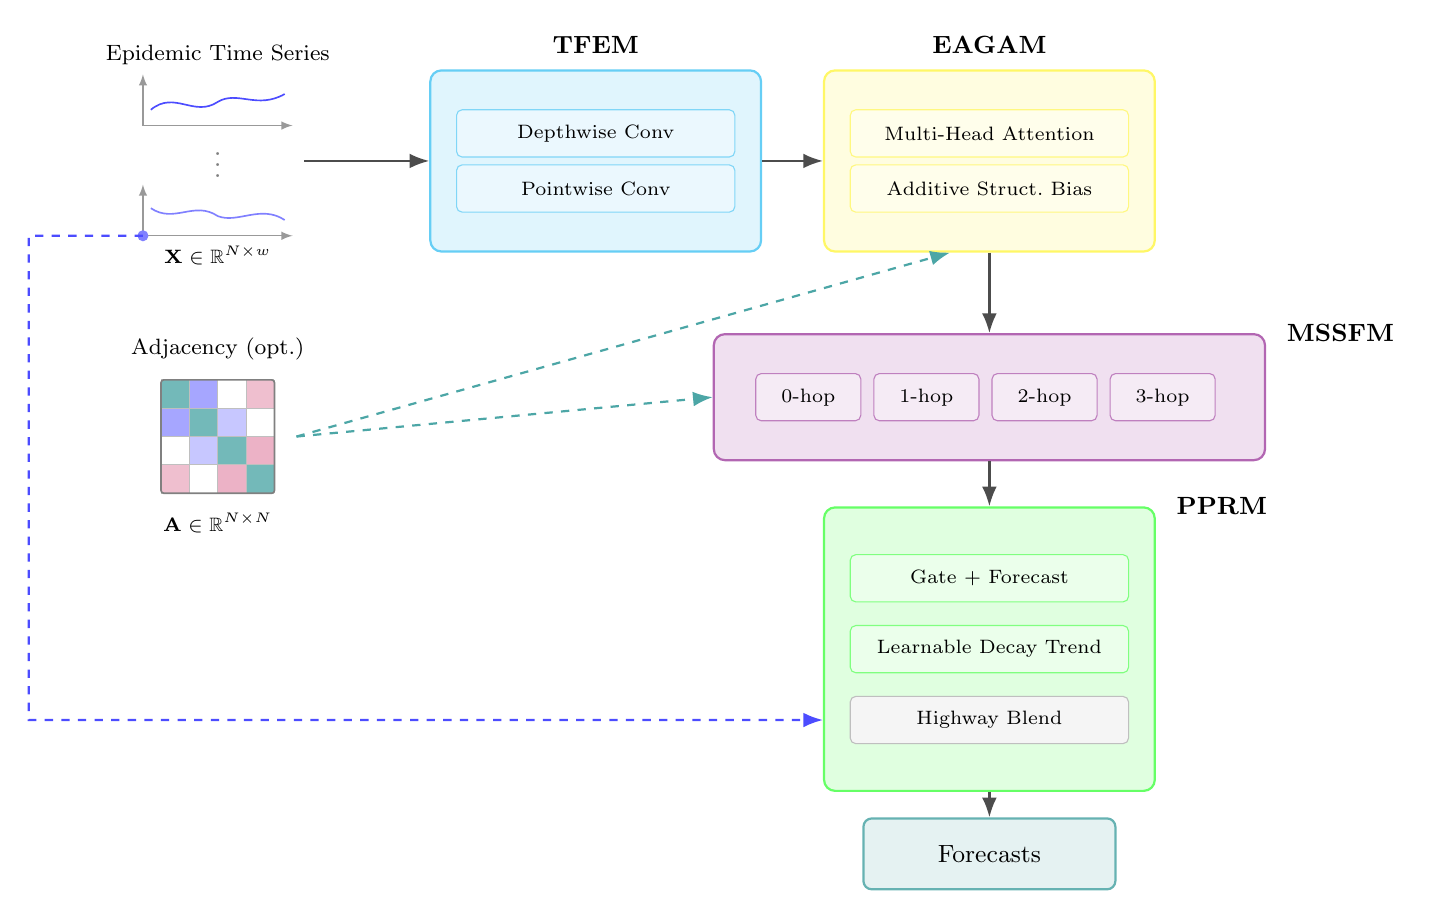
\begin{tikzpicture}[
        font=\scriptsize,
        >=latex,
        % --- Styles ---
        sblock/.style={
            rectangle, draw=#1!50, rounded corners=2pt,
            minimum height=0.6cm, text width=3.3cm,
            align=center, fill=#1!8, font=\scriptsize
        },
        iobox/.style={
            rectangle, draw=#1!60, thick, rounded corners=3pt,
            minimum height=0.9cm, minimum width=3.0cm,
            align=center, fill=#1!10, font=\small
        },
        modwrap/.style={
            rectangle, draw=#1!60, thick, rounded corners=4pt,
            align=center, fill=#1!12, inner sep=7pt
        },
        arr/.style={-{Latex[length=2.5mm]}, thick, black!70},
        darr/.style={-{Latex[length=2.5mm]}, dashed, thick, #1!70},
        lbl/.style={font=\small\bfseries, black}
    ]

    % ============================================================
    %  INPUT:  Two mini time-series plots with axes, dots between
    % ============================================================
    % --- Top time series (Region 1) ---
    \begin{scope}[shift={(-5.8, 0.7)}]
        \draw[->, black!40, thin] (-0.95, -0.25) -- (0.95, -0.25);
        \draw[->, black!40, thin] (-0.95, -0.25) -- (-0.95, 0.4);
        \draw[blue!70, semithick]
            (-0.85, -0.05)
            .. controls (-0.55, 0.2) and (-0.3, -0.15) .. (0.0, 0.05)
            .. controls (0.25, 0.2) and (0.5, -0.05) .. (0.85, 0.15);
    \end{scope}
    % --- Dots (regions 2 to N-1) ---
    \node[black!50, font=\normalsize] at (-5.8, 0.05) {$\vdots$};
    % --- Bottom time series (Region N) ---
    \begin{scope}[shift={(-5.8, -0.7)}]
        \draw[->, black!40, thin] (-0.95, -0.25) -- (0.95, -0.25);
        \draw[->, black!40, thin] (-0.95, -0.25) -- (-0.95, 0.4);
        \draw[blue!50, semithick]
            (-0.85, 0.1)
            .. controls (-0.55, -0.1) and (-0.3, 0.2) .. (0.0, 0.0)
            .. controls (0.25, -0.1) and (0.55, 0.15) .. (0.85, -0.05);
    \end{scope}
    \node[font=\footnotesize] at (-5.8, 1.35) {Epidemic Time Series};
    \node[font=\scriptsize] at (-5.8, -1.2) {$\mathbf{X}\in\mathbb{R}^{N\times w}$};
    \coordinate (IN) at (-4.7, 0);

    % ============================================================
    %  TFEM  (wider boxes so text fits)
    % ============================================================
    \node[modwrap=cyan, minimum height=2.3cm, minimum width=4.2cm] (tfem) at (-1.0, 0) {};
    \node[lbl, above=2pt of tfem] {TFEM};
    \node[sblock=cyan] (dw) at ([yshift=0.35cm]tfem.center) {Depthwise Conv};
    \node[sblock=cyan] (pw) at ([yshift=-0.35cm]tfem.center) {Pointwise Conv};

    % ============================================================
    %  EAGAM  (wider boxes so text fits)
    % ============================================================
    \node[modwrap=yellow, minimum height=2.3cm, minimum width=4.2cm] (eagam) at (4.0, 0) {};
    \node[lbl, above=2pt of eagam] {EAGAM};
    \node[sblock=yellow] (mha) at ([yshift=0.35cm]eagam.center) {Multi-Head Attention};
    \node[sblock=yellow] (srb) at ([yshift=-0.35cm]eagam.center) {Additive Struct.\ Bias};

    % Row 1 arrows
    \draw[arr] (IN) -- (tfem);
    \draw[arr] (tfem) -- (eagam);

    % ============================================================
    %  MSSFM  (label shifted right, away from arrow)
    % ============================================================
    \node[modwrap=violet, minimum height=1.6cm, minimum width=7.0cm]
        (mssfm) at (4.0, -3.0) {};
    \node[lbl, right=4pt] at (mssfm.north east) {MSSFM};
    \node[sblock=violet, text width=1.1cm] at ([xshift=-2.3cm]mssfm.center) {0-hop};
    \node[sblock=violet, text width=1.1cm] at ([xshift=-0.8cm]mssfm.center) {1-hop};
    \node[sblock=violet, text width=1.1cm] at ([xshift=0.7cm]mssfm.center)  {2-hop};
    \node[sblock=violet, text width=1.1cm] at ([xshift=2.2cm]mssfm.center)  {3-hop};

    \draw[arr] (eagam) -- (mssfm);

    % ============================================================
    %  PPRM  (includes Highway Blend; label shifted right)
    % ============================================================
    \node[modwrap=green, minimum height=3.6cm, minimum width=4.2cm]
        (pprm) at (4.0, -6.2) {};
    \node[lbl, right=4pt] at (pprm.north east) {PPRM};
    \node[sblock=green] (gf) at ([yshift=0.9cm]pprm.center)  {Gate + Forecast};
    \node[sblock=green] (dt) at (pprm.center)                 {Learnable Decay Trend};
    \node[sblock=gray]  (hw) at ([yshift=-0.9cm]pprm.center)  {Highway Blend};

    \draw[arr] (mssfm) -- (pprm);

    % ============================================================
    %  OUTPUT
    % ============================================================
    \node[iobox=teal, minimum width=3.2cm] (output) at (4.0, -8.8) {Forecasts};

    \draw[arr] (pprm) -- (output);

    % ============================================================
    %  ADJACENCY ICON  (heatmap-style matrix, multi-colour)
    % ============================================================
    \begin{scope}[shift={(-5.8, -3.5)}]
        \def\cs{0.36}          % cell size
        \def\ox{-0.72}         % grid left  = -4 half-cells
        \def\oy{-0.72}         % grid bottom
        %
        % --- Cell fills (symmetric matrix; diagonal = self-connection) ---
        % Row 0 (top row, i=0)
        \fill[teal!55]   (\ox,         \oy+3*\cs) rectangle +(\cs,\cs);  % (0,0) diag
        \fill[blue!35]   (\ox+\cs,     \oy+3*\cs) rectangle +(\cs,\cs);  % (0,1)
        \fill[white]     (\ox+2*\cs,   \oy+3*\cs) rectangle +(\cs,\cs);  % (0,2)
        \fill[purple!25] (\ox+3*\cs,   \oy+3*\cs) rectangle +(\cs,\cs);  % (0,3)
        % Row 1
        \fill[blue!35]   (\ox,         \oy+2*\cs) rectangle +(\cs,\cs);  % (1,0) sym
        \fill[teal!55]   (\ox+\cs,     \oy+2*\cs) rectangle +(\cs,\cs);  % (1,1) diag
        \fill[blue!22]   (\ox+2*\cs,   \oy+2*\cs) rectangle +(\cs,\cs);  % (1,2)
        \fill[white]     (\ox+3*\cs,   \oy+2*\cs) rectangle +(\cs,\cs);  % (1,3)
        % Row 2
        \fill[white]     (\ox,         \oy+\cs)   rectangle +(\cs,\cs);  % (2,0)
        \fill[blue!22]   (\ox+\cs,     \oy+\cs)   rectangle +(\cs,\cs);  % (2,1) sym
        \fill[teal!55]   (\ox+2*\cs,   \oy+\cs)   rectangle +(\cs,\cs);  % (2,2) diag
        \fill[purple!30] (\ox+3*\cs,   \oy+\cs)   rectangle +(\cs,\cs);  % (2,3)
        % Row 3 (bottom)
        \fill[purple!25] (\ox,         \oy)        rectangle +(\cs,\cs);  % (3,0) sym
        \fill[white]     (\ox+\cs,     \oy)        rectangle +(\cs,\cs);  % (3,1)
        \fill[purple!30] (\ox+2*\cs,   \oy)        rectangle +(\cs,\cs);  % (3,2) sym
        \fill[teal!55]   (\ox+3*\cs,   \oy)        rectangle +(\cs,\cs);  % (3,3) diag
        %
        % --- Grid lines ---
        \foreach \i in {0,...,4} {
            \draw[black!25, thin] (\ox+\i*\cs, \oy) -- (\ox+\i*\cs, \oy+4*\cs);
            \draw[black!25, thin] (\ox, \oy+\i*\cs) -- (\ox+4*\cs, \oy+\i*\cs);
        }
        % Outer border
        \draw[black!50, semithick, rounded corners=1pt]
            (\ox,\oy) rectangle (\ox+4*\cs, \oy+4*\cs);
        %
        \node[font=\footnotesize, above] at (0, 0.85) {Adjacency (opt.)};
        \node[font=\scriptsize, below] at (0, -0.85) {$\mathbf{A}\in\mathbb{R}^{N\times N}$};
    \end{scope}
    \coordinate (ADJ) at (-4.8, -3.5);

    % ============================================================
    %  ADJACENCY ARROWS  (clean diagonals, no crossing)
    % ============================================================
    \draw[darr=teal] (ADJ) -- ([xshift=-0.5cm]eagam.south);
    \draw[darr=teal] (ADJ) -- (mssfm.west);

    % ============================================================
    %  AUTOREGRESSIVE SKIP  (far-left route into Highway sub-block)
    % ============================================================
    \fill[blue!50] (-6.75, -0.95) circle (2pt);
    \draw[darr=blue]
        (-6.75, -0.95) -- (-8.2, -0.95) -- (-8.2, -7.1) -- ([yshift=-0.9cm]pprm.west);

    \end{tikzpicture}%
    }
    \caption{Overview of the MSAGAT-Net architecture. Epidemic time series pass through TFEM, EAGAM, MSSFM, and PPRM before producing forecasts. Teal dashed lines: optional adjacency matrix; blue dashed line: autoregressive skip connection into the Highway Blend.}
    \label{fig:msagat_net_architecture}
\end{figure}

\subsection{Temporal Feature Extraction Module (TFEM)}

The first component of the MSAGAT-Net architecture is TFEM, which transforms the raw time-series data into compact feature representations. Given input data $\mathbf{X} = [\mathbf{x}_{t-w+1}, \ldots, \mathbf{x}_t] \in \mathbb{R}^{N \times w}$ for $N$ regions over a look-back window of $w$ time steps, TFEM extracts temporal features through depthwise separable convolutions \cite{chollet2017xception} followed by low-rank projections, reducing parameter count and computational cost while maintaining expressive power \cite{li2023multi, yu2022traffic}.

\subsubsection{Depthwise Separable Convolutions}

For each region's historical window $\mathbf{x}^i_{[t-w+1:t]} \in \mathbb{R}^w$, we apply a depthwise convolution followed by a pointwise convolution. The depthwise convolution applies a separate filter per channel:

\begin{equation}
\mathbf{z}^i_{\text{depth}} = \text{Conv1D}_{\text{depth}}(\mathbf{x}^i; \boldsymbol{\Theta}_{\text{depth}})
\end{equation}

where $\mathbf{z}^i_{\text{depth}} \in \mathbb{R}^{w \times 1}$ represents the output after depthwise convolution, preserving the temporal dimension while processing each input channel independently.

Following the depthwise convolution, a pointwise convolution (implemented as a 1×1 convolution) is applied to expand the single channel to multiple feature channels:

\begin{equation}
\mathbf{z}^i_{\text{point}} = \text{Conv1D}_{\text{point}}(\mathbf{z}^i_{\text{depth}}; \boldsymbol{\Theta}_{\text{point}})
\end{equation}

where $\mathbf{z}^i_{\text{point}} \in \mathbb{R}^{w \times d_{\text{feat}}}$ and $d_{\text{feat}} = 16$ is the number of output feature channels. Batch normalisation and ReLU activation are applied after each convolution:

\begin{equation}
\mathbf{z}^i_{\text{norm}} = \text{ReLU}(\text{BatchNorm}(\mathbf{z}^i_{\text{point}}))
\end{equation}

\subsubsection{Low-Rank Feature Projection}

After extracting features using depthwise separable convolutions, we applied a low-rank projection to further reduce dimensionality and capture the most salient features. This projection consists of two linear transformations with a bottleneck in between:

\begin{equation}
\mathbf{F}^i_{\text{low}} = \text{Linear}_{\text{low}}(\text{Flatten}(\mathbf{z}^i_{\text{norm}}))
\end{equation}

\begin{equation}
\mathbf{F}^i = \text{Linear}_{\text{high}}(\mathbf{F}^i_{\text{low}})
\end{equation}

where $\mathbf{F}^i_{\text{low}} \in \mathbb{R}^{d_{\text{bottle}}}$ denotes the bottleneck representation and $\mathbf{F}^i \in \mathbb{R}^{d_{\text{hidden}}}$ is the final feature vector for region $i$. The flattening operation maps $\mathbf{z}^i_{\text{norm}} \in \mathbb{R}^{w \times d_{\text{feat}}}$ to a vector of dimension $w d_{\text{feat}}$, which is then compressed through the bottleneck ($d_{\text{bottle}} \ll w d_{\text{feat}}$) before being expanded to dimension $d_{\text{hidden}}$. This low-rank bottleneck reduces the parameter count per region from $\mathcal{O}(w \cdot d_{\text{feat}} \cdot d_{\text{hidden}})$ to $\mathcal{O}(w \cdot d_{\text{feat}} \cdot d_{\text{bottle}} + d_{\text{bottle}} \cdot d_{\text{hidden}})$, while also regularising the representation by forcing the model to preserve only the most predictive temporal patterns.

Applying this projection to all regions produces the feature matrix $\mathbf{F} \in \mathbb{R}^{N \times d_{\text{hidden}}}$, followed by layer normalisation and ReLU activation.

\begin{equation}
\mathbf{F} = \text{ReLU}(\text{LayerNorm}(\mathbf{F}))
\end{equation}

The TFEM pipeline is illustrated in Figure~\ref{fig:feature_extraction}.

All hyperparameters of TFEM ($d_{\text{feat}}$, $d_{\text{bottle}}$, $d_{\text{hidden}}$, kernel size) are reported in Table~\ref{tab:hyperparameters}.

\begin{figure}[!htbp]
\centering
\resizebox{1.0\linewidth}{!}{%
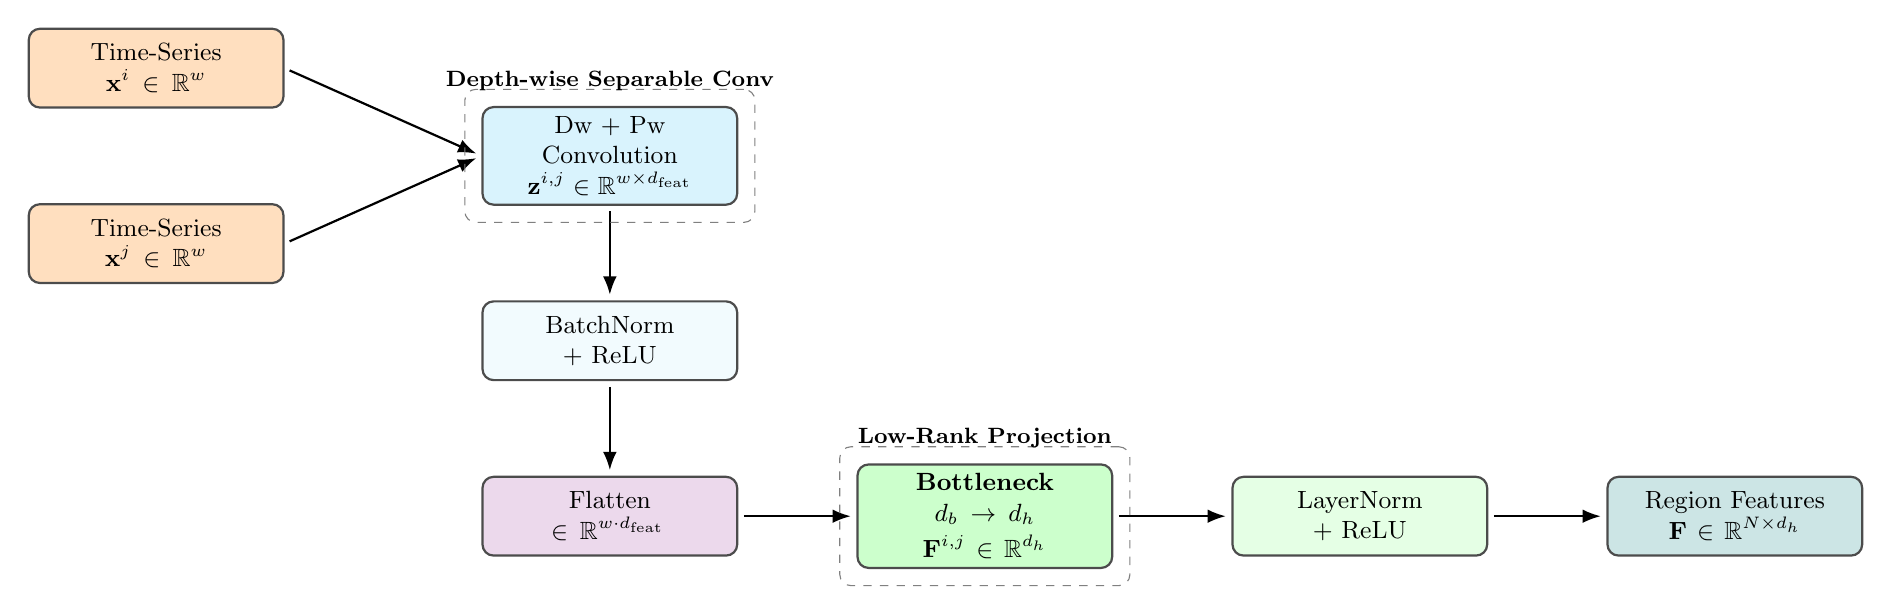
\begin{tikzpicture}[
    font=\small,
    >=Latex,
    block/.style={
        rectangle, draw=black!70, thick,
        rounded corners, align=center,
        minimum height=1cm,  % Increased height
        text width=3cm       % Increased width
    },
    arrow/.style={->, thick, shorten >=2pt, shorten <=2pt},
]
  %––– Inputs (split) –––––––––––––––––––––––––––––––––––––––
  \node (xi) [block, fill=orange!25] {Time‑Series\\$\mathbf{x}^i\!\in\!\mathbb{R}^{w}$};
  \node (xj) [block, fill=orange!25, below=1.2cm of xi] {Time‑Series\\$\mathbf{x}^j\!\in\!\mathbb{R}^{w}$};

  % Compute a point centred between xi and xj for tidy piping
  \path (xi.east) -- (xj.east) coordinate[midway] (midinput);

  %––– Pipeline nodes –––––––––––––––––––––––––––––––––––––––
  \node (sepconv) [block, fill=cyan!15,  right=2.5cm of midinput] {
      Dw + Pw\\Convolution\\
      $\mathbf{z}^{i,j}\!\in\!\mathbb{R}^{w\times d_{\text{feat}}}$};

  \node (bn)   [block, fill=cyan!5, below=1.2cm of sepconv] {BatchNorm\\+ ReLU};

  \node (flat) [block, fill=violet!15, below=1.2cm of bn] {Flatten\\$\!\in\!\mathbb{R}^{w\cdot d_{\text{feat}}}$};

  % Horizontal arrangement for the remaining nodes
  \node (proj) [block, fill=green!20, right=1.5cm of flat] {
      \textbf{Bottleneck}\\$d_b\!\to\! d_h$\\[2pt]
      $\mathbf{F}^{i,j}\!\in\!\mathbb{R}^{d_{h}}$};

  \node (ln) [block, fill=green!10, right=1.5cm of proj] {LayerNorm\\+ ReLU};

  \node (output) [block, fill=teal!20, right=1.5cm of ln] {Region Features\\$\mathbf{F}\!\in\!\mathbb{R}^{N\times d_{h}}$};

  %––– Arrows –––––––––––––––––––––––––––––––––––––––––––––––
  \draw[arrow] (xi.east) -- (sepconv.west);
  \draw[arrow] (xj.east) -- (sepconv.west);
  \draw[arrow] (sepconv.south) -- ++(0,-0.6) -- (bn.north);
  \draw[arrow] (bn.south) -- ++(0,-0.6) -- (flat.north);
  \draw[arrow] (flat.east) -- (proj.west);
  \draw[arrow] (proj.east) -- (ln.west);
  \draw[arrow] (ln.east) -- (output.west);

  %––– Grouping boxes –––––––––––––––––––––––––––––––––––––––
  % \begin{scope}[on background layer] % Removed for IEEEtran compatibility
    \node[draw=black!50, dashed, rounded corners, inner sep=6pt,
          fit=(sepconv)] {};
    \node at (sepconv.north) [above=2pt, font=\footnotesize\bfseries] {Depth‑wise Separable Conv};

    \node[draw=black!50, dashed, rounded corners, inner sep=6pt,
          fit=(proj)] {};
    \node at (proj.north) [above=2pt, font=\footnotesize\bfseries] {Low‑Rank Projection};
  % \end{scope} % Removed for IEEEtran compatibility
\end{tikzpicture}%
}
\caption{TFEM feature-extraction pipeline. Regional time series are processed through depthwise separable convolutions, flattened, and passed through a low-rank bottleneck to yield region-level feature vectors $\mathbf{F}$.}
\label{fig:feature_extraction}
\end{figure}

\subsection{Efficient Adaptive Graph Attention with Low-Rank Decomposition}

The second core component of MSAGAT-Net is the Efficient Adaptive Graph Attention Module (EAGAM). Conventional spatial modelling approaches rely on fixed adjacency matrices, which cannot fully capture the evolving nature of epidemic spread. Building on graph attention networks \cite{velickovic2017graph}, EAGAM learns inter-regional relationships directly from feature representations rather than being restricted to a predefined graph structure. However, standard graph attention mechanisms incur $\mathcal{O}(N^2 \cdot d)$ complexity and do not provide a principled way to regulate how strongly a structural prior influences learnt attention. The Low-rank decomposition offers an effective way to reduce the cost of the parameters \cite{puny2020global, kong2023low, yang2023self}, motivating the design of EAGAM.

EAGAM uses multi-head scaled dot-product attention with low-rank bottleneck projections for the query, key, and value representations. Its central innovation is the incorporation of two complementary structural biases directly into the attention scores \emph{before} softmax normalisation: (i) a learnable low-rank graph bias $\mathbf{B} = \mathbf{UV}$ that captures persistent spatial relationships from the data, and (ii) an optional additive adjacency prior to a learnable scale whose influence self-attenuates with graph density, as detailed in Section~\ref{sec:adj_prior}. The module consists of five components, described in the following.


\subsubsection{Bottleneck Projection}

Given the feature matrix $\mathbf{F} \in \mathbb{R}^{N \times d_{\text{hidden}}}$ from TFEM, where $N$ is the number of regions and $d_{\text{hidden}}$ is the hidden dimension, we first project these features into query, key, and value representations through an efficient bottleneck projection:

\begin{equation}
\mathbf{Q}_{\text{low}}, \mathbf{K}_{\text{low}}, \mathbf{V}_{\text{low}} = \text{Split}(\text{Linear}_{\text{low}}(\mathbf{F}), 3)
\end{equation}

where $\text{Linear}_{\text{low}}: \mathbb{R}^{d_{\text{hidden}}} \rightarrow \mathbb{R}^{3 \times d_{\text{bottle}}}$ projects the features into a lower-dimensional space and $\text{Split}$ divides the output into three separate tensors of dimension $\mathbb{R}^{N \times d_{\text{bottle}}}$.

These low-dimensional projections are then expanded back to the full hidden dimension:

\begin{equation}
\mathbf{Q}, \mathbf{K}, \mathbf{V} = \text{Split}(\text{Linear}_{\text{high}}([\mathbf{Q}_{\text{low}}; \mathbf{K}_{\text{low}}; \mathbf{V}_{\text{low}}]), 3)
\end{equation}

where $\text{Linear}_{\text{high}}: \mathbb{R}^{3 \times d_{\text{bottle}}} \rightarrow \mathbb{R}^{3 \times d_{\text{hidden}}}$ and each of $\mathbf{Q}, \mathbf{K}, \mathbf{V} \in \mathbb{R}^{N \times d_{\text{hidden}}}$.

This bottleneck projection significantly reduces the parameter count from $\mathcal{O}(3 \times d_{\text{hidden}}^2)$ to $\mathcal{O}(3 \times d_{\text{hidden}} \times d_{\text{bottle}})$, where $d_{\text{bottle}} \ll d_{\text{hidden}}$.

\subsubsection{Multi-Head Attention Mechanism}

To capture different types of inter-regional relationships, we employ multi-head attention with $H$ heads, each of dimension $d_{\text{head}} = d_{\text{hidden}} / H$. The query, key and value matrices are reshaped into $[H, N, d_{\text{head}}]$ tensors. For each head $m \in \{1, \ldots, H\}$, we computed scaled dot-product attention scores:

\begin{equation}
\mathbf{S}^{(m)} = \frac{\mathbf{Q}^{(m)} {\mathbf{K}^{(m)}}^T}{\sqrt{d_{\text{head}}}}
\end{equation}

where $\mathbf{S}^{(m)} \in \mathbb{R}^{N \times N}$. Two structural biases, a learnable graph bias $\mathbf{B}^{(m)}$ (Section~\ref{sec:graph_bias}) and an optional adjacency prior (Section~\ref{sec:adj_prior}), are added before softmax normalisation:

\begin{equation}
\mathbf{A}^{(m)} = \text{softmax}(\mathbf{S}^{(m)} + \mathbf{B}^{(m)} + \alpha \cdot \tilde{\mathbf{A}})
\end{equation}

where $\mathbf{B}^{(m)}$ is the $m$-th head slice of the learnable graph bias $\mathbf{B} = \mathbf{UV}$, $\tilde{\mathbf{A}}$ is the row-normalised adjacency prior (when available) and $\alpha = \text{softplus}(\alpha_0)$ is a learnable positive scale parameter. The self-attenuating properties of this additive formulation are analysed in Section~\ref{sec:adj_prior}.

The final attention output for each head is then computed as:

\begin{equation}
\mathbf{O}^{(m)} = \mathbf{A}^{(m)} \mathbf{V}^{(m)}
\end{equation}

where $\mathbf{O}^{(m)} \in \mathbb{R}^{N \times d_{\text{head}}}$. The outputs of all $H$ heads are concatenated and projected back to $d_{\text{hidden}}$.

\subsubsection{Learnable Graph Structure Bias}
\label{sec:graph_bias}

Unlike traditional graph attention networks that rely solely on node features to compute attention \cite{velickovic2017graph}, EAGAM includes a learnable bias term that captures persistent structural relationships between regions. This bias is implemented as a low-rank decomposition for parameter efficiency:

\begin{equation}
\mathbf{B} = \mathbf{U} \mathbf{V}
\end{equation}

where $\mathbf{U} \in \mathbb{R}^{h \times N \times d_{\text{bias}}}$ and $\mathbf{V} \in \mathbb{R}^{h \times d_{\text{bias}} \times N}$ are learnable parameters initialised with the Xavier uniform \cite{glorot2010understanding}, and $d_{\text{bias}} \ll N$ is the bottleneck dimension. The resulting bias $\mathbf{B} \in \mathbb{R}^{h \times N \times N}$ is added directly to content-based attention scores before softmax, allowing it to reinforce or suppress specific region-to-region attention patterns as a first-class component of the spatial reasoning mechanism.

\subsubsection{Self-Attenuating Additive Adjacency Prior}
\label{sec:adj_prior}

Unlike state-of-the-art baselines that \emph{require} predefined adjacency matrices, MSAGAT-Net learns spatial relationships entirely from data. When prior knowledge about regional connectivity is available (e.g., geographical proximity or mobility patterns), it can optionally be incorporated through an additive prior mechanism to accelerate learning and improve performance.

Given an adjacency matrix $\mathbf{A}$, we first compute a row-normalised prior:

\begin{equation}
\tilde{\mathbf{A}} = \mathbf{D}_{\text{row}}^{-1}\mathbf{A}
\end{equation}

where $\mathbf{D}_{\text{row}} = \text{diag}(\mathbf{A}\mathbf{1})$ is the diagonal matrix of the sum of the rows. This prior is then added to the attention scores with a learnable positive scale:

\begin{equation}
\mathbf{S}_h' = \mathbf{S}_h + \mathbf{B} + \alpha \cdot \tilde{\mathbf{A}}
\end{equation}

where $\alpha = \text{softplus}(\alpha_0)$ ensures positivity, and $\alpha_0$ is a learnable scalar parameter initialised to $1.0$ (yielding $\alpha \approx 1.31$ initially, providing a moderate structural nudge).

The key insight behind this additive formulation is its \emph{self-attenuating} behaviour across different graph topologies. Because the softmax function is shift-invariant, i.e., $\text{softmax}(\mathbf{x} + c\mathbf{1}) = \text{softmax}(\mathbf{x})$ for any constant vector $c\mathbf{1}$, the prior's effect is attenuated when the row-normalised adjacency approaches a uniform distribution:

\begin{itemize}
    \item \textbf{Dense graphs:} When the adjacency matrix is dense and the degrees of the nodes are relatively uniform, the prior normalised to the row $\tilde{\mathbf{A}}$ approaches a nearly uniform distribution across columns. Adding a near-constant vector to each row of attention scores before softmax has a negligible effect on the resulting attention distribution, so the model relies primarily on content-based attention and the learnt graph bias.
    \item \textbf{Sparse graphs:} When the adjacency matrix is sparse, $\tilde{\mathbf{A}}$ has peaked entries for connected nodes and zeros elsewhere. The additive prior meaningfully shifts attention towards geographically relevant neighbours, providing structural guidance where it is most needed.
\end{itemize}

This self-attenuating property eliminates the need for graph-size-dependent thresholds or conditional gating mechanisms, which we found to be fragile in practice. When no adjacency is provided, the model operates using only content-based attention and the learnt graph bias; when adjacency is available, the scale $\alpha$ is learnt during training, and the prior is pre-computed and stored as a constant buffer with negligible overhead. This distinguishes MSAGAT-Net from baselines such as EpiGNN \cite{xie2022epignn}, Cola-GNN \cite{dengColaGNNCrosslocationAttention2020a}, and DCRNN \cite{li2017diffusion}, which mandate adjacency matrices as required input. Figure~\ref{fig:self_regulating} illustrates this mechanism with a concrete example.

\begin{figure}[!ht]
\centering
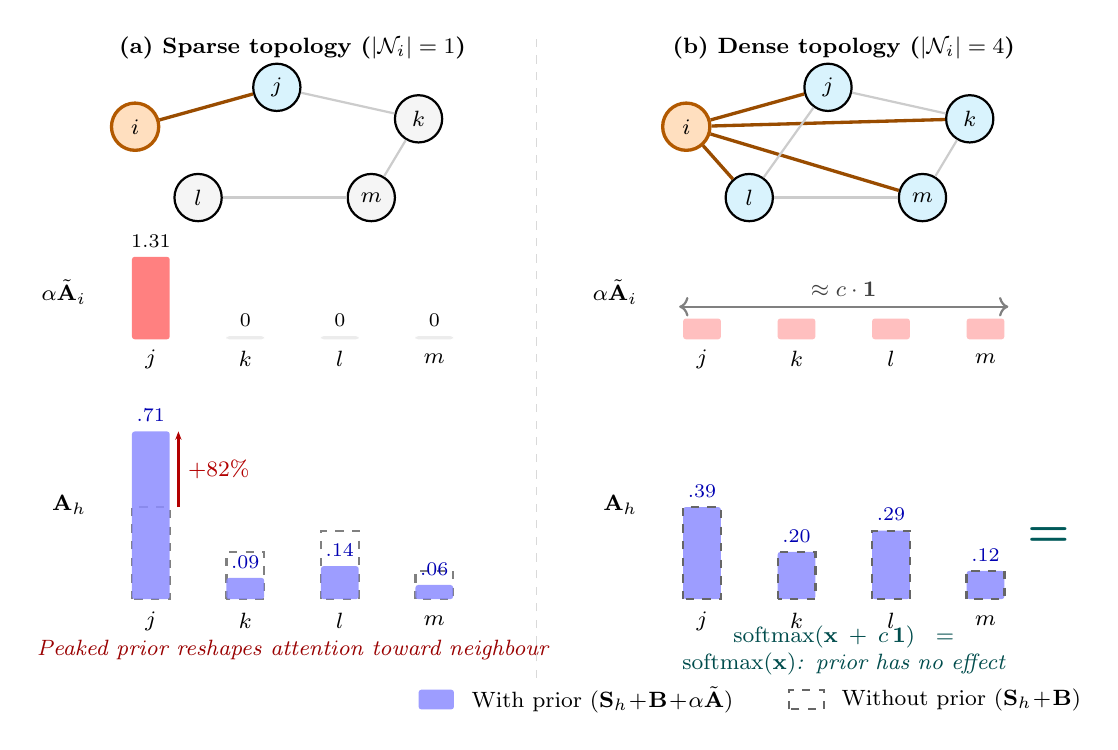
\begin{tikzpicture}[font=\footnotesize,
    gnode/.style={circle, draw, thick, minimum size=6mm, inner sep=0pt, font=\footnotesize},
    inode/.style={gnode, fill=orange!25, draw=orange!70!black, line width=1.2pt},
    cnode/.style={gnode, fill=cyan!15},
    unode/.style={gnode, fill=gray!8},
    iedge/.style={very thick, orange!60!black},
    oedge/.style={thick, black!20},
    barlbl/.style={font=\footnotesize},
    vallbl/.style={font=\scriptsize, above, blue!70!black},
]

% Bar x-positions (shared across panels)
\pgfmathsetmacro{\xa}{1.4}
\pgfmathsetmacro{\xb}{2.6}
\pgfmathsetmacro{\xc}{3.8}
\pgfmathsetmacro{\xd}{5.0}
\pgfmathsetmacro{\hw}{0.24}
% Vertical scales
\pgfmathsetmacro{\pscale}{0.8}   % prior bar scale
\pgfmathsetmacro{\ascale}{3.0}   % attention bar scale

%% ======== PANEL (a): SPARSE ========
\begin{scope}
  \node[font=\footnotesize\bfseries] at (3.2,7.4) {(a) Sparse topology ($|\mathcal{N}_i|=1$)};

  %-- Graph --
  \node[inode] (i1) at (1.2,6.4) {$i$};
  \node[cnode] (j1) at (3.0,6.9) {$j$};
  \node[unode] (k1) at (4.8,6.5) {$k$};
  \node[unode] (l1) at (2.0,5.5) {$l$};
  \node[unode] (m1) at (4.2,5.5) {$m$};
  \draw[iedge] (i1)--(j1);
  \draw[oedge] (j1)--(k1);
  \draw[oedge] (k1)--(m1);
  \draw[oedge] (l1)--(m1);

  %-- Row-normalised adjacency prior --
  \node[font=\footnotesize, anchor=east] at (0.7,4.3) {$\alpha\tilde{\mathbf{A}}_i$};
  \fill[red!50, rounded corners=1pt] (\xa-\hw,3.7) rectangle (\xa+\hw,3.7+1.31*\pscale);
  \fill[gray!15, rounded corners=1pt] (\xb-\hw,3.7) rectangle (\xb+\hw,3.74);
  \fill[gray!15, rounded corners=1pt] (\xc-\hw,3.7) rectangle (\xc+\hw,3.74);
  \fill[gray!15, rounded corners=1pt] (\xd-\hw,3.7) rectangle (\xd+\hw,3.74);
  \node[font=\scriptsize, above] at (\xa,3.7+1.31*\pscale) {$1.31$};
  \node[font=\scriptsize, above] at (\xb,3.74) {$0$};
  \node[font=\scriptsize, above] at (\xc,3.74) {$0$};
  \node[font=\scriptsize, above] at (\xd,3.74) {$0$};
  \node[barlbl] at (\xa,3.45) {$j$};
  \node[barlbl] at (\xb,3.45) {$k$};
  \node[barlbl] at (\xc,3.45) {$l$};
  \node[barlbl] at (\xd,3.45) {$m$};

  %-- Resulting attention distribution --
  \node[font=\footnotesize, anchor=east] at (0.7,1.6) {$\mathbf{A}_h$};
  % Dashed outlines = without prior: softmax([1.5,0.8,1.2,0.3]) = [0.39, 0.20, 0.29, 0.12]
  \draw[black!50, dashed, thick] (\xa-\hw,0.4) rectangle (\xa+\hw,0.4+0.39*\ascale);
  \draw[black!50, dashed, thick] (\xb-\hw,0.4) rectangle (\xb+\hw,0.4+0.20*\ascale);
  \draw[black!50, dashed, thick] (\xc-\hw,0.4) rectangle (\xc+\hw,0.4+0.29*\ascale);
  \draw[black!50, dashed, thick] (\xd-\hw,0.4) rectangle (\xd+\hw,0.4+0.12*\ascale);
  % Filled = with prior: softmax([2.81,0.8,1.2,0.3]) = [0.71, 0.09, 0.14, 0.06]
  \fill[blue!45, opacity=0.85, rounded corners=1pt] (\xa-\hw,0.4) rectangle (\xa+\hw,0.4+0.71*\ascale);
  \fill[blue!45, opacity=0.85, rounded corners=1pt] (\xb-\hw,0.4) rectangle (\xb+\hw,0.4+0.09*\ascale);
  \fill[blue!45, opacity=0.85, rounded corners=1pt] (\xc-\hw,0.4) rectangle (\xc+\hw,0.4+0.14*\ascale);
  \fill[blue!45, opacity=0.85, rounded corners=1pt] (\xd-\hw,0.4) rectangle (\xd+\hw,0.4+0.06*\ascale);
  % Value labels on bars
  \node[vallbl] at (\xa,0.4+0.71*\ascale) {.71};
  \node[vallbl] at (\xb,0.4+0.09*\ascale) {.09};
  \node[vallbl] at (\xc,0.4+0.14*\ascale) {.14};
  \node[vallbl] at (\xd,0.4+0.06*\ascale) {.06};
  \node[barlbl] at (\xa,0.12) {$j$};
  \node[barlbl] at (\xb,0.12) {$k$};
  \node[barlbl] at (\xc,0.12) {$l$};
  \node[barlbl] at (\xd,0.12) {$m$};

  % Change arrow on node j
  \draw[-{Stealth[length=3pt]}, very thick, red!70!black] (\xa+0.35,0.4+0.39*\ascale) -- (\xa+0.35,0.4+0.71*\ascale);
  \node[font=\footnotesize, red!70!black, right] at (\xa+0.35,0.4+0.55*\ascale) {+82\%};

  \node[font=\footnotesize\itshape, text=red!60!black] at (3.2,-0.25)
    {Peaked prior reshapes attention toward neighbour};
\end{scope}

%% ======== DIVIDER ========
\draw[gray!30, dashed] (6.3,-0.6) -- (6.3,7.6);

%% ======== PANEL (b): DENSE ========
\begin{scope}[shift={(7.0,0)}]
  \node[font=\footnotesize\bfseries] at (3.2,7.4) {(b) Dense topology ($|\mathcal{N}_i|=4$)};

  %-- Graph --
  \node[inode] (i2) at (1.2,6.4) {$i$};
  \node[cnode] (j2) at (3.0,6.9) {$j$};
  \node[cnode] (k2) at (4.8,6.5) {$k$};
  \node[cnode] (l2) at (2.0,5.5) {$l$};
  \node[cnode] (m2) at (4.2,5.5) {$m$};
  \draw[iedge] (i2)--(j2);
  \draw[iedge] (i2)--(k2);
  \draw[iedge] (i2)--(l2);
  \draw[iedge] (i2)--(m2);
  \draw[oedge] (j2)--(k2);
  \draw[oedge] (l2)--(m2);
  \draw[oedge] (j2)--(l2);
  \draw[oedge] (k2)--(m2);

  %-- Row-normalised adjacency prior (near-uniform) --
  \node[font=\footnotesize, anchor=east] at (0.7,4.3) {$\alpha\tilde{\mathbf{A}}_i$};
  \fill[red!25, rounded corners=1pt] (\xa-\hw,3.7) rectangle (\xa+\hw,3.7+0.33*\pscale);
  \fill[red!25, rounded corners=1pt] (\xb-\hw,3.7) rectangle (\xb+\hw,3.7+0.33*\pscale);
  \fill[red!25, rounded corners=1pt] (\xc-\hw,3.7) rectangle (\xc+\hw,3.7+0.33*\pscale);
  \fill[red!25, rounded corners=1pt] (\xd-\hw,3.7) rectangle (\xd+\hw,3.7+0.33*\pscale);
  \draw[<->, gray, thick] (\xa-\hw-0.05,3.7+0.33*\pscale+0.15) -- (\xd+\hw+0.05,3.7+0.33*\pscale+0.15);
  \node[font=\footnotesize, gray!50!black, above] at (3.2,3.7+0.33*\pscale+0.15) {$\approx c\cdot\mathbf{1}$};
  \node[barlbl] at (\xa,3.45) {$j$};
  \node[barlbl] at (\xb,3.45) {$k$};
  \node[barlbl] at (\xc,3.45) {$l$};
  \node[barlbl] at (\xd,3.45) {$m$};

  %-- Resulting attention distribution (identical with and without prior) --
  \node[font=\footnotesize, anchor=east] at (0.7,1.6) {$\mathbf{A}_h$};
  % Filled bars: [0.39, 0.20, 0.29, 0.12]
  \fill[blue!45, opacity=0.85, rounded corners=1pt] (\xa-\hw,0.4) rectangle (\xa+\hw,0.4+0.39*\ascale);
  \fill[blue!45, opacity=0.85, rounded corners=1pt] (\xb-\hw,0.4) rectangle (\xb+\hw,0.4+0.20*\ascale);
  \fill[blue!45, opacity=0.85, rounded corners=1pt] (\xc-\hw,0.4) rectangle (\xc+\hw,0.4+0.29*\ascale);
  \fill[blue!45, opacity=0.85, rounded corners=1pt] (\xd-\hw,0.4) rectangle (\xd+\hw,0.4+0.12*\ascale);
  % Dashed outlines on top (without prior -- identical heights, clearly visible)
  \draw[black!60, dashed, thick] (\xa-\hw,0.4) rectangle (\xa+\hw,0.4+0.39*\ascale);
  \draw[black!60, dashed, thick] (\xb-\hw,0.4) rectangle (\xb+\hw,0.4+0.20*\ascale);
  \draw[black!60, dashed, thick] (\xc-\hw,0.4) rectangle (\xc+\hw,0.4+0.29*\ascale);
  \draw[black!60, dashed, thick] (\xd-\hw,0.4) rectangle (\xd+\hw,0.4+0.12*\ascale);
  % Value labels on bars
  \node[vallbl] at (\xa,0.4+0.39*\ascale) {.39};
  \node[vallbl] at (\xb,0.4+0.20*\ascale) {.20};
  \node[vallbl] at (\xc,0.4+0.29*\ascale) {.29};
  \node[vallbl] at (\xd,0.4+0.12*\ascale) {.12};
  \node[barlbl] at (\xa,0.12) {$j$};
  \node[barlbl] at (\xb,0.12) {$k$};
  \node[barlbl] at (\xc,0.12) {$l$};
  \node[barlbl] at (\xd,0.12) {$m$};

  % Prominent equality annotation
  \node[teal!70!black, scale=2.0] at (5.8,1.2) {$\boldsymbol{=}$};

  \node[font=\footnotesize\itshape, text=teal!60!black, text width=5.5cm, align=center] at (3.2,-0.25)
    {$\mathrm{softmax}(\mathbf{x}+c\,\mathbf{1})=\mathrm{softmax}(\mathbf{x})$: prior has no effect};
\end{scope}

%% ======== LEGEND (centered) ========
\fill[blue!45, opacity=0.85, rounded corners=1pt] (4.8,-1.0) rectangle (5.25,-0.75);
\node[font=\footnotesize, right] at (5.35,-0.875) {With prior $(\mathbf{S}_h\!+\!\mathbf{B}\!+\!\alpha\tilde{\mathbf{A}})$};
\draw[black!60, dashed, thick] (9.5,-1.0) rectangle (9.95,-0.75);
\node[font=\footnotesize, right] at (10.05,-0.875) {Without prior $(\mathbf{S}_h\!+\!\mathbf{B})$};

\end{tikzpicture}
\caption{Self-attenuating behaviour of the additive adjacency prior for node~$i$, with identical content scores in both panels. \textbf{(a)}~Sparse graph: peaked prior redistributes attention toward neighbour~$j$. \textbf{(b)}~Dense graph: near-uniform prior has no effect after softmax.}
\label{fig:self_regulating}
\end{figure}

\subsubsection{Attention Regularisation}

Attention sparsity is promoted implicitly through three mechanisms: (i) the low-rank bottleneck projections for queries and keys constrain the effective rank of the attention matrix, (ii) the learnable graph bias $\mathbf{B} = \mathbf{UV}$ concentrates attention on structurally relevant pairs, and (iii) the L2 weight decay applied to all parameters (via the Adam optimiser) penalises large attention logits. Together, these encourage sparse and interpretable attention patterns without requiring an explicit sparsity penalty term in the loss function.

The head outputs $\{\mathbf{O}^{(1)}, \ldots, \mathbf{O}^{(H)}\}$ are concatenated and reshaped into $\mathbf{O} \in \mathbb{R}^{N \times d_{\text{hidden}}}$. We then employ a low-rank output projection for efficiency:

\begin{equation}
\mathbf{O}_{\text{low}} = \text{Linear}_{\text{out\_low}}(\mathbf{O})
\end{equation}

\begin{equation}
\mathbf{O}_{\text{final}} = \text{Linear}_{\text{out\_high}}(\mathbf{O}_{\text{low}})
\end{equation}

where $\mathbf{O}_{\text{low}} \in \mathbb{R}^{N \times d_{\text{bottle}}}$ and $\mathbf{O}_{\text{final}} \in \mathbb{R}^{N \times d_{\text{hidden}}}$.

The output of EAGAM, $\mathbf{O}_{\text{final}}$, represents the features of each region after incorporating spatial dependencies, and is passed to the subsequent MSSFM for further processing.

All EAGAM hyperparameters (attention heads, bottleneck dimension, regularisation weight, adjacency prior scale) are reported in Table~\ref{tab:hyperparameters}. Figure~\ref{fig:eagam_module} presents the data flow through the EAGAM module.

\begin{figure}[!ht]
\centering
\resizebox{0.72\linewidth}{!}{%
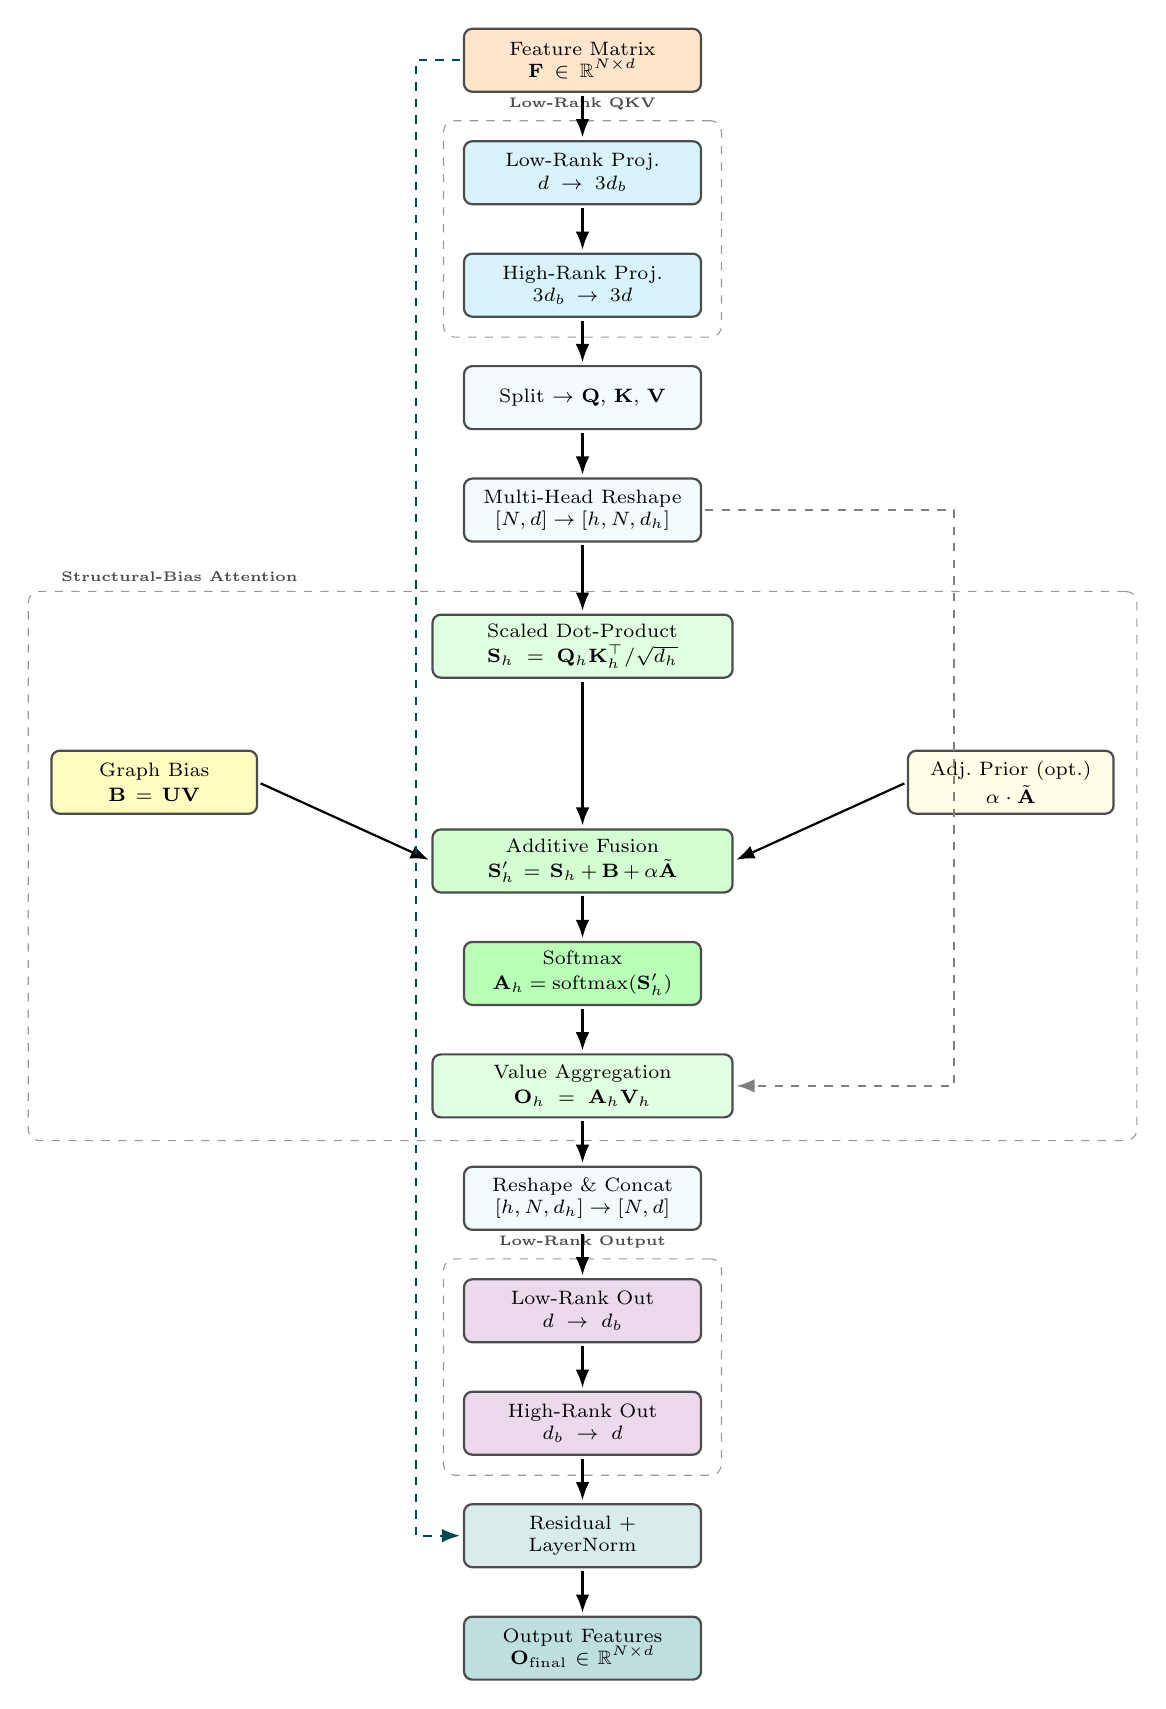
\begin{tikzpicture}[
    font=\scriptsize,
    >=Latex,
    node distance = 0.6cm and 1.4cm,
    % --- node styles ---
    block/.style = {rectangle, draw=black!70, thick,
                    rounded corners=3pt, align=center,
                    minimum height=0.8cm,
                    text width=2.8cm,
                    inner sep=3pt},
    wblock/.style = {block, text width=3.6cm},
    sideblock/.style = {block, text width=2.4cm},
    arrow/.style  = {->, thick, shorten >=1pt, shorten <=1pt},
    darrow/.style = {->, thick, dashed, shorten >=1pt, shorten <=1pt},
    grouplbl/.style = {font=\tiny\bfseries, text=black!70},
]

%============ INPUT ============
\node (input) [block, fill=orange!20]
  {Feature Matrix\\$\mathbf{F}\!\in\!\mathbb{R}^{N\times d}$};

%============ LOW-RANK QKV PROJECTION ============
\node (qkv_low) [block, fill=cyan!15, below=of input]
  {Low-Rank Proj.\\$d \!\to\! 3d_b$};

\node (qkv_high) [block, fill=cyan!15, below=of qkv_low]
  {High-Rank Proj.\\$3d_b \!\to\! 3d$};

\node (split) [block, fill=cyan!5, below=of qkv_high]
  {Split $\to$ $\mathbf{Q}$, $\mathbf{K}$, $\mathbf{V}$};

\node (reshape) [block, fill=cyan!5, below=of split]
  {Multi-Head Reshape\\$[N,d]\!\to\![h,N,d_h]$};

%============ CONTENT ATTENTION ============
\node (dotprod) [wblock, fill=green!12, below=0.9cm of reshape]
  {Scaled Dot-Product\\[1pt]
   $\mathbf{S}_h = \mathbf{Q}_h\mathbf{K}_h^\top / \sqrt{d_h}$};

%============ STRUCTURAL BIASES (side branches) ============
\node (gbias) [sideblock, fill=yellow!25, below left=0.9cm and 2.2cm of dotprod]
  {Graph Bias\\[1pt]$\mathbf{B}\!=\!\mathbf{U}\mathbf{V}$};

\node (adjpr) [sideblock, fill=yellow!10, below right=0.9cm and 2.2cm of dotprod]
  {Adj.\ Prior (opt.)\\[1pt]$\alpha\!\cdot\!\tilde{\mathbf{A}}$};

%============ ADDITIVE FUSION ============
\node (addfuse) [wblock, fill=green!18, below=1.9cm of dotprod]
  {Additive Fusion\\[1pt]
   $\mathbf{S}_h'\!=\!\mathbf{S}_h\!+\!\mathbf{B}\!+\!\alpha\tilde{\mathbf{A}}$};

%============ SOFTMAX ============
\node (softmax) [block, fill=green!28, below=of addfuse]
  {Softmax\\[1pt]
   $\mathbf{A}_h\!=\!\mathrm{softmax}(\mathbf{S}_h')$};

%============ VALUE AGGREGATION ============
\node (valagg) [wblock, fill=green!12, below=of softmax]
  {Value Aggregation\\[1pt]
   $\mathbf{O}_h\!=\!\mathbf{A}_h\mathbf{V}_h$};

%============ (regularisation node removed) ============

%============ OUTPUT PATH ============
\node (reshapeout) [block, fill=cyan!5, below=of valagg]
  {Reshape \& Concat\\$[h,N,d_h]\!\to\![N,d]$};

\node (outlow) [block, fill=violet!15, below=of reshapeout]
  {Low-Rank Out\\$d\!\to\! d_b$};

\node (outhigh) [block, fill=violet!15, below=of outlow]
  {High-Rank Out\\$d_b\!\to\! d$};

\node (resid) [block, fill=teal!15, below=of outhigh]
  {Residual + LayerNorm};

\node (output) [block, fill=teal!25, below=of resid]
  {Output Features\\$\mathbf{O}_{\mathrm{final}}\!\in\!\mathbb{R}^{N\times d}$};

%============ MAIN-FLOW ARROWS ============
\foreach \a/\b in {
  input/qkv_low, qkv_low/qkv_high, qkv_high/split, split/reshape,
  reshape/dotprod, dotprod/addfuse,
  addfuse/softmax, softmax/valagg,
  valagg/reshapeout, reshapeout/outlow, outlow/outhigh, outhigh/resid, resid/output}
  \draw[arrow] (\a) -- (\b);

% Structural-bias arrows into additive fusion
\draw[arrow] (gbias.east)  -- (addfuse.west);
\draw[arrow] (adjpr.west)  -- (addfuse.east);

% (regularisation arrow removed)

% V path bypass (dashed): from reshape directly to value aggregation
\draw[darrow, gray] (reshape.east) -- ++(3.2,0) |- (valagg.east);

% Residual skip connection from input to residual+LN node
\draw[darrow, teal!60!black]
  (input.west) -- ++(-0.6,0) |- (resid.west);

%============ GROUP BOXES (background) ============
\begin{scope}[on background layer]
  % Low-Rank QKV group
  \node [draw=black!40, dashed, rounded corners=4pt, inner sep=7pt,
         fit=(qkv_low)(qkv_high), label={[grouplbl]above:Low-Rank QKV}] {};

  % Structural-Bias Attention group
  \node [draw=black!40, dashed, rounded corners=4pt, inner sep=8pt,
         fit=(dotprod)(gbias)(adjpr)(addfuse)(softmax)(valagg),
         label={[grouplbl]above left:Structural-Bias Attention}] {};

  % Low-Rank Output group
  \node [draw=black!40, dashed, rounded corners=4pt, inner sep=7pt,
         fit=(outlow)(outhigh), label={[grouplbl]above:Low-Rank Output}] {};
\end{scope}

\end{tikzpicture}}%
\caption{Data flow in the EAGAM module. Input features $\mathbf{F}$ are projected through a low-rank bottleneck into Q, K, V representations. Scaled dot-product scores are augmented with a learnable graph bias $\mathbf{B}=\mathbf{UV}$ and an optional adjacency prior $\alpha\cdot\tilde{\mathbf{A}}$ before softmax. Attended values pass through a low-rank output stage with residual connection.}
\label{fig:eagam_module}
\end{figure}

\subsection{Multi-Scale Spatial Feature Module}
\label{sec:mssfm}

The third major component of the proposed MSAGAT-Net architecture is MSSFM, which refines spatial dependencies using multi-hop graph convolutions. Epidemic propagation involves interactions that extend beyond immediate neighbours, but excessive diffusion can oversmooth small graphs \cite{li2018deeper}. MSSFM addresses this by aggregating information across multiple hop distances while adaptively limiting the maximum hop depth based on graph size and fusing scales with locality-biased weights.

\subsubsection{Multi-Hop Graph Convolutions}

Let $\mathbf{G} \in \mathbb{R}^{B \times N \times d_{\text{hidden}}}$ denote the spatial features produced by EAGAM. Given an adjacency matrix $\mathbf{A}$, we construct a row-normalised matrix with self-loops:

\begin{equation}
\mathbf{\hat{A}} = \mathbf{D}^{-1}(\mathbf{A} + \mathbf{I}),
\end{equation}

where $\mathbf{D}$ is the degree matrix of $(\mathbf{A} + \mathbf{I})$. For each hop $k \in \{0, 1, \ldots, S-1\}$, MSSFM computes a k-hop aggregation:

\begin{equation}
\mathbf{H}^{(k)} = \mathbf{\hat{A}}^{k}\mathbf{G}\mathbf{W}^{(k)},
\end{equation}

with $\mathbf{W}^{(k)}$ implemented as a linear transform followed by LayerNorm and ReLU. The $k=0$ scale uses the identity matrix to preserve self-features. When no adjacency is provided, MSSFM defaults to identity aggregation across all scales.

\subsubsection{Adaptive Hop Depth and Locality-Biased Fusion}

To reduce oversmoothing on small graphs, the number of scales is set adaptively as
\begin{equation}
S = \min(S_{\max}, \max(2, \lfloor N/5 \rfloor)),
\end{equation}
ensuring that small graphs use fewer hops, while larger graphs retain broader context (yielding $S=2$ for Australia-COVID ($N{=}8$), NHS-ICUBeds ($N{=}7$) and US-Regions ($N{=}10$), and $S=4$ for Japan-Prefectures ($N{=}47$), US-States ($N{=}49$) and LTLA-COVID ($N{=}372$)). We fuse the multi-hop features with learnable weights initialised to favour locality:

\begin{equation}
w_k^{(0)} = \exp(-0.5\,k), \quad
\boldsymbol{\alpha} = \text{softmax}(\mathbf{w}), \quad
\mathbf{H}_{\text{fused}} = \sum_{k=0}^{S-1} \alpha_k \mathbf{H}^{(k)}.
\end{equation}

The exponential initialisation assigns higher initial weight to lower hops (e.g.\ $\alpha_0 > \alpha_1 > \alpha_2 > \alpha_3$), encoding a locality prior that the model can override during training if longer-range dependencies become informative.

\subsubsection{Bottleneck Projection and Residual Connection}

The fused features are passed through a low-rank bottleneck projection and residual connection to stabilise training:

\begin{equation}
\mathbf{H}_{\text{proj}} = \text{Linear}_{\text{high}}(\text{Linear}_{\text{low}}(\mathbf{H}_{\text{fused}})),
\end{equation}
\begin{equation}
\mathbf{H}_{\text{final}} = \text{LayerNorm}(\mathbf{H}_{\text{proj}} + \mathbf{G}).
\end{equation}

This design preserves the hidden dimension while enabling adaptive spatial refinement over multiple hop distances. Figure~\ref{fig:mssfm_module} illustrates the flow of data through the MSSFM module.

\begin{figure}[!htbp]
\centering
\resizebox{0.78\linewidth}{!}{%
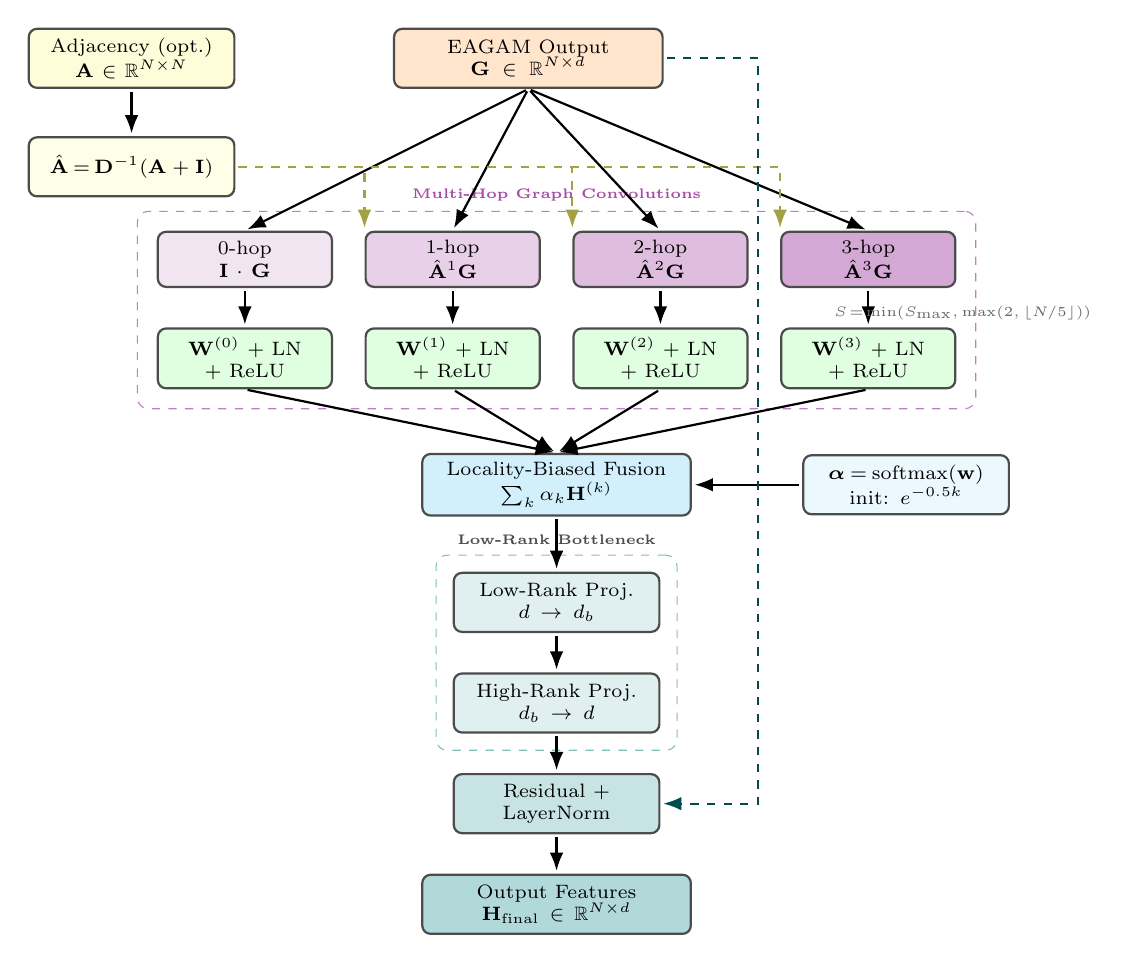
\begin{tikzpicture}[
    font=\scriptsize,
    >=Latex,
    node distance = 0.55cm and 1.0cm,
    % --- node styles ---
    block/.style = {rectangle, draw=black!70, thick,
                    rounded corners=3pt, align=center,
                    minimum height=0.75cm,
                    text width=2.4cm,
                    inner sep=3pt},
    wblock/.style = {block, text width=3.2cm},
    hopblock/.style = {block, minimum height=0.7cm, text width=2.0cm},
    arrow/.style  = {->, thick, shorten >=1pt, shorten <=1pt},
    darrow/.style = {->, thick, dashed, shorten >=1pt, shorten <=1pt},
    grouplbl/.style = {font=\tiny\bfseries, text=black!70},
]

%============ INPUT ============
\node (input) [wblock, fill=orange!20]
  {EAGAM Output\\$\mathbf{G}\!\in\!\mathbb{R}^{N\times d}$};

%============ ADJACENCY ============
\node (adj) [block, fill=yellow!15, left=2.0cm of input]
  {Adjacency (opt.)\\$\mathbf{A}\!\in\!\mathbb{R}^{N\times N}$};

\node (adjhat) [block, fill=yellow!10, below=0.6cm of adj]
  {$\hat{\mathbf{A}}\!=\!\mathbf{D}^{-1}(\mathbf{A}+\mathbf{I})$};

\draw[arrow] (adj) -- (adjhat);

%============ PARALLEL HOP BRANCHES ============
% Position them below the input, spaced horizontally
\node (hop0) [hopblock, fill=violet!10, below=1.8cm of input, xshift=-3.6cm]
  {0-hop\\$\mathbf{I}\cdot\mathbf{G}$};
\node (hop1) [hopblock, fill=violet!18, right=0.4cm of hop0]
  {1-hop\\$\hat{\mathbf{A}}^1\mathbf{G}$};
\node (hop2) [hopblock, fill=violet!26, right=0.4cm of hop1]
  {2-hop\\$\hat{\mathbf{A}}^2\mathbf{G}$};
\node (hop3) [hopblock, fill=violet!34, right=0.4cm of hop2]
  {3-hop\\$\hat{\mathbf{A}}^3\mathbf{G}$};

% Input feeds all hops
\foreach \h in {hop0,hop1,hop2,hop3}
  \draw[arrow] (input.south) -- (\h.north);

% Adjacency powers feed hops 1--3
\draw[darrow, yellow!60!black] (adjhat.east) -| (hop1.north west);
\draw[darrow, yellow!60!black] (adjhat.east) -| (hop2.north west);
\draw[darrow, yellow!60!black] (adjhat.east) -| (hop3.north west);

%============ PER-HOP TRANSFORMS ============
\node (w0) [hopblock, fill=green!12, below=0.5cm of hop0]
  {$\mathbf{W}^{(0)}$ + LN + ReLU};
\node (w1) [hopblock, fill=green!12, below=0.5cm of hop1]
  {$\mathbf{W}^{(1)}$ + LN + ReLU};
\node (w2) [hopblock, fill=green!12, below=0.5cm of hop2]
  {$\mathbf{W}^{(2)}$ + LN + ReLU};
\node (w3) [hopblock, fill=green!12, below=0.5cm of hop3]
  {$\mathbf{W}^{(3)}$ + LN + ReLU};

\foreach \h/\w in {hop0/w0, hop1/w1, hop2/w2, hop3/w3}
  \draw[arrow] (\h) -- (\w);

%============ ADAPTIVE FUSION ============
\node (fusion) [wblock, fill=cyan!18, below=1.2cm of $(w1)!0.5!(w2)$]
  {Locality-Biased Fusion\\$\sum_k \alpha_k \mathbf{H}^{(k)}$};

\foreach \w in {w0,w1,w2,w3}
  \draw[arrow] (\w.south) -- (fusion.north);

% Alpha weights annotation
\node (alpha) [block, fill=cyan!8, right=1.4cm of fusion]
  {$\boldsymbol{\alpha}\!=\!\mathrm{softmax}(\mathbf{w})$\\init: $e^{-0.5k}$};
\draw[arrow] (alpha) -- (fusion);

%============ BOTTLENECK + RESIDUAL ============
\node (bnlow) [block, fill=teal!12, below=0.7cm of fusion]
  {Low-Rank Proj.\\$d\!\to\! d_b$};

\node (bnhigh) [block, fill=teal!12, below=0.5cm of bnlow]
  {High-Rank Proj.\\$d_b\!\to\! d$};

\node (resid) [block, fill=teal!22, below=0.5cm of bnhigh]
  {Residual + LayerNorm};

\node (output) [wblock, fill=teal!30, below=0.5cm of resid]
  {Output Features\\$\mathbf{H}_{\mathrm{final}}\!\in\!\mathbb{R}^{N\times d}$};

\foreach \a/\b in {fusion/bnlow, bnlow/bnhigh, bnhigh/resid, resid/output}
  \draw[arrow] (\a) -- (\b);

% Residual skip from input to residual+LN
\draw[darrow, teal!60!black]
  (input.east) -- ++(1.2,0) |- (resid.east);

%============ ADAPTIVE HOP DEPTH ANNOTATION ============
\node [font=\tiny, text=black!60, align=center,
       below=0.1cm of hop3, xshift=1.2cm]
  {$S\!=\!\min(S_{\max},\max(2,\lfloor N/5\rfloor))$};

%============ GROUP BOXES ============
\begin{scope}[on background layer]
  % Multi-hop branches group
  \node [draw=violet!50, dashed, rounded corners=4pt, inner sep=7pt,
         fit=(hop0)(hop3)(w0)(w3),
         label={[grouplbl, text=violet!70]above:Multi-Hop Graph Convolutions}] {};

  % Bottleneck group
  \node [draw=teal!50, dashed, rounded corners=4pt, inner sep=6pt,
         fit=(bnlow)(bnhigh),
         label={[grouplbl]above:Low-Rank Bottleneck}] {};
\end{scope}

\end{tikzpicture}}%
\caption{Data flow in the MSSFM module. Parallel multi-hop branches ($\hat{\mathbf{A}}^0$ to $\hat{\mathbf{A}}^{S-1}$) are fused with locality-biased weights and projected through a low-rank bottleneck with a residual connection.}
\label{fig:mssfm_module}
\end{figure}


\subsection{Progressive Multi-Horizon Forecast Refinement}

The final component of the MSAGAT-Net architecture is the Progressive Prediction Refinement Module (PPRM). Forecast errors tend to accumulate over longer horizons \cite{BENTAIEB20127067, chandra2021evaluation}; accordingly, PPRM introduces an adaptive refinement mechanism, inspired by gating principles in recurrent networks \cite{hochreiter1997long}, that balances model-based forecasts with trend-based extrapolations derived from recent observations.


\subsubsection{Low-Rank Forecast Projection}

Given the spatiotemporal feature tensor $\mathbf{H}_{\text{final}} \in \mathbb{R}^{B \times N \times d_{\text{hidden}}}$ from MSSFM, where $B$ is the batch size, $N$ is the number of regions, and $d_{\text{hidden}}$ is the hidden dimension, we first apply a bottleneck projection to distil the most forecast-relevant information:

\begin{equation}
\mathbf{P}_{\text{low}} = \text{Linear}_{\text{pred\_low}}(\mathbf{H}_{\text{final}})
\end{equation}

where $\mathbf{P}_{\text{low}} \in \mathbb{R}^{B \times N \times d_{\text{bottle}}}$ is the bottleneck representation with dimension $d_{\text{bottle}} \ll d_{\text{hidden}}$. This projection reduces dimensionality before the final forecast layer, lowering the parameter count while encouraging compact feature representations.

We then apply layer normalisation, ReLU activation, and dropout to the bottleneck representation:

\begin{equation}
\mathbf{P}_{\text{mid}} = \text{Dropout}(\text{ReLU}(\text{LayerNorm}(\mathbf{P}_{\text{low}})))
\end{equation}

\subsubsection{Horizon-Specific Forecasting}

From the processed bottleneck representation, we generate initial forecasts for all forecast horizons using a linear projection:

\begin{equation}
\mathbf{P}_{\text{initial}} = \text{Linear}_{\text{pred\_high}}(\mathbf{P}_{\text{mid}})
\end{equation}

where $\mathbf{P}_{\text{initial}} \in \mathbb{R}^{B \times N \times h}$ represents the raw model forecasts for each region across all forecast horizons $h$.

\subsubsection{Adaptive Refinement Mechanism}

To improve multi-horizon stability, the initial forecasts are combined with trend-based extrapolations from recent observations through a learned gating mechanism. We first compute an adaptive gate based on the spatiotemporal features:

\begin{equation}
\mathbf{R} = \sigma(\text{Linear}_{\text{gate\_high}}(\text{ReLU}(\text{Linear}_{\text{gate\_low}}(\mathbf{H}_{\text{final}}))))
\end{equation}

where $\mathbf{R} \in \mathbb{R}^{B \times N \times h}$ represents gate values between 0 and 1 for each region and forecast horizon, and $\sigma$ denotes the sigmoid activation function.

We use the most recent observation $\mathbf{x}_{\text{last}} \in \mathbb{R}^{B \times N}$ to generate a trend-based forecast using an exponential decay projection with a \emph{learnable} decay rate:

\begin{equation}
\mathbf{T} = \mathbf{x}_{\text{last}} \odot \exp(-\gamma \cdot \mathbf{d}), \quad \gamma = \exp(\gamma_0)
\end{equation}

where $\mathbf{x}_{\text{last}}$ is expanded to the shape $[B, N, h]$, $\mathbf{d} \in \mathbb{R}^h$ is a vector of increasing horizon indices $[1, 2, \ldots, h]$, $\gamma_0$ is a learnable scalar parameter stored in log-domain to ensure positivity (initialised to $-2.3$, yielding $\gamma \approx 0.1$ at the start of training), and $\odot$ represents element-wise multiplication.

This exponential decay formulation is inspired by epidemiological models that exhibit exponential growth or decay patterns. Crucially, the decay rate $\gamma$ is learned during training rather than fixed, allowing the model to adapt the trend extrapolation speed to each dataset's dynamics, with faster decay for rapidly changing epidemics and slower decay for more persistent trends.

The final forecasts are then computed as a weighted combination of the model-based forecasts and the trend-based projections:

\begin{equation}
\mathbf{P}_{\text{final}} = \mathbf{R} \odot \mathbf{P}_{\text{initial}} + (1 - \mathbf{R}) \odot \mathbf{T}
\end{equation}

where $\mathbf{P}_{\text{final}} \in \mathbb{R}^{B \times N \times h}$ represents the refined forecasts for each region across all forecast horizons.

All PPRM hyperparameters ($d_{\text{bottle}}$, $\gamma_0$, dropout) are reported in Table~\ref{tab:hyperparameters}. The forecast horizon $h$ is configurable, and we evaluate $h \in \{3, 5, 7, 10, 14, 15\}$ across our experiments.


\begin{figure}[hb]
\centering
% ~0.55·textheight; width adapts automatically
\resizebox{!}{0.55\textheight}{%
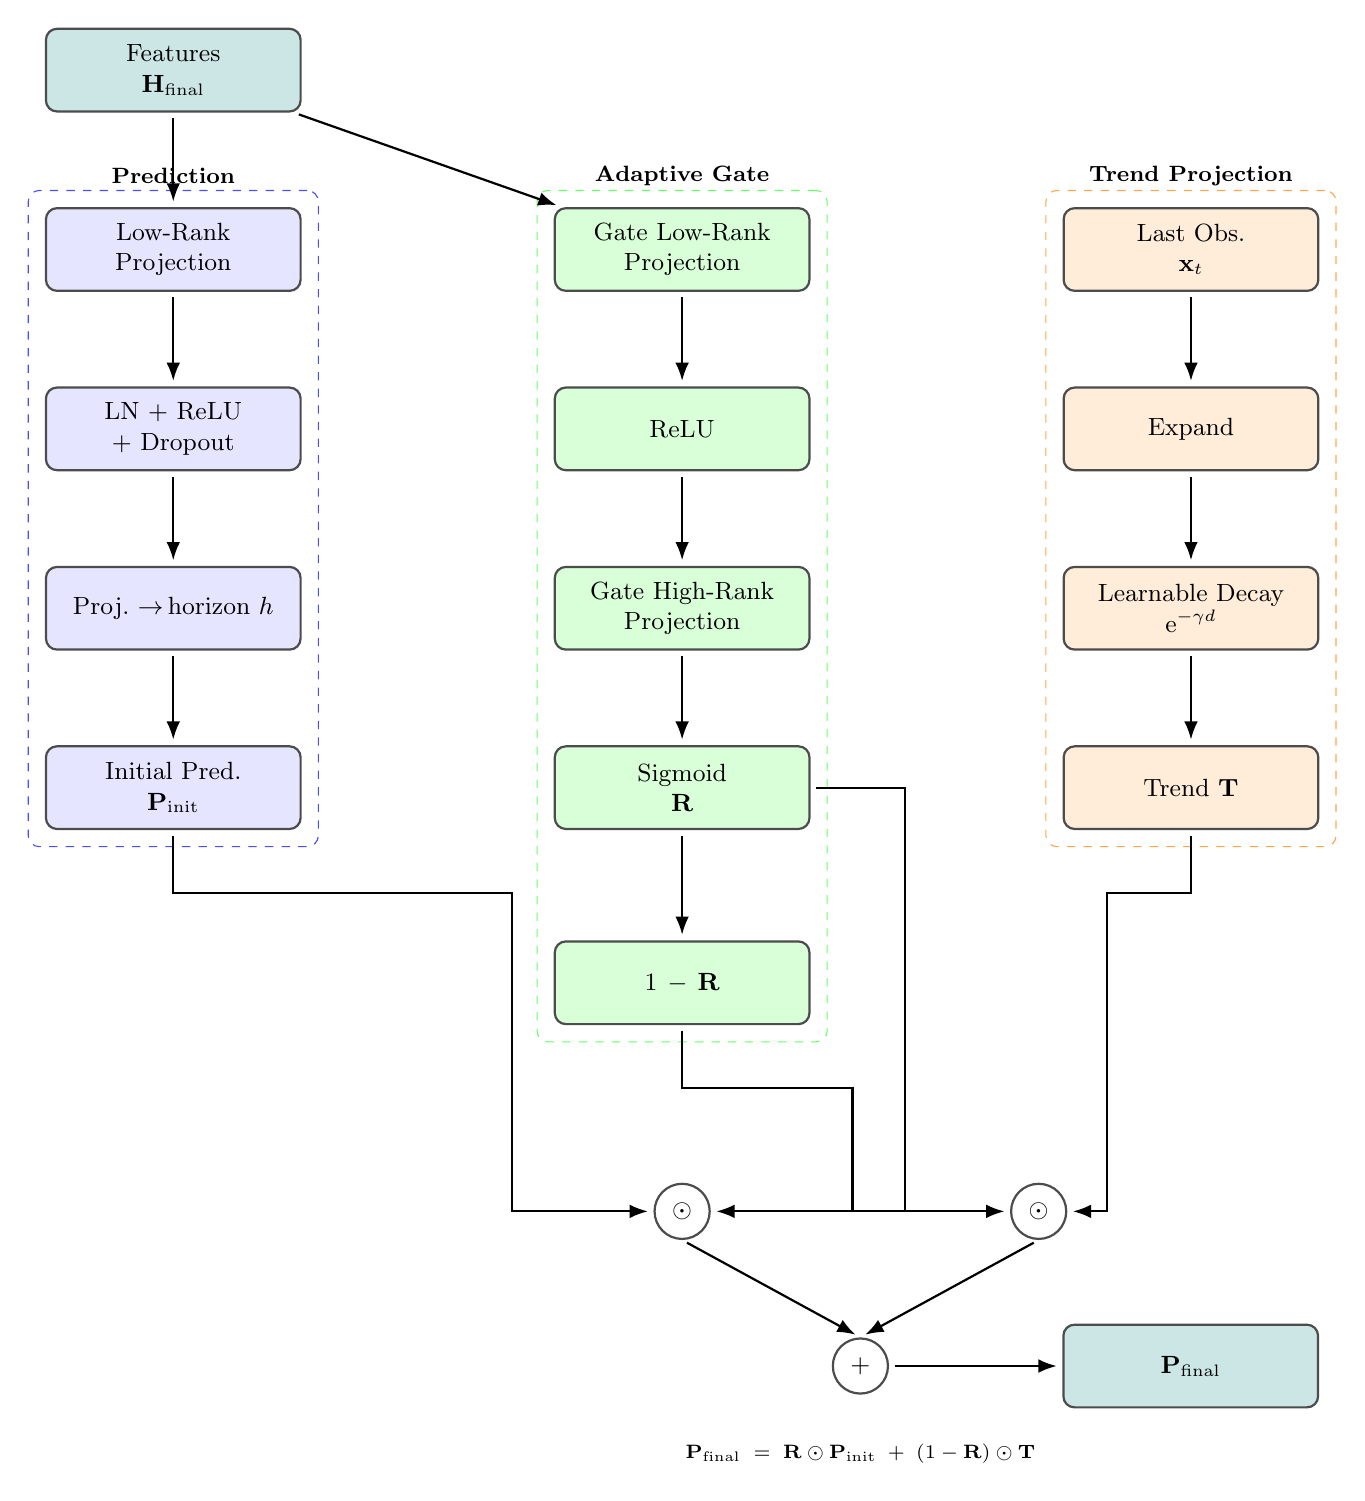
\begin{tikzpicture}[
    font=\small,
    >=Latex,
    node distance = 1.2cm and 1.8cm,
    block/.style={rectangle, draw=black!70, thick,
                  rounded corners, align=center,
                  minimum height=1.05cm, text width=3.0cm},
    pred/.style ={block, fill=blue!10},
    gate/.style ={block, fill=green!15},
    trend/.style={block, fill=orange!15},
    io/.style   ={block, fill=teal!20},
    op/.style   ={circle, draw=black!70, thick,
                  minimum size=0.7cm, inner sep=0pt},
    arrow/.style={->, thick, shorten >=2pt, shorten <=2pt}
]

%–––– INPUT –––––––––––––––––––––––––––––––––––––––––
\node (input) [io] {Features\\$\mathbf H_{\text{final}}$};

%–––– PREDICTION PATH ––––––––––––––––––––––––––––––
\node (plow)  [pred, below=of input]        {Low‑Rank\\Projection};
\node (pmid)  [pred, below=of plow]         {LN + ReLU + Dropout};
\node (phigh) [pred, below=of pmid]         {Proj. $\!\to\!$ horizon $h$};
\node (pinit) [pred, below=of phigh]        {Initial Pred.\\$\mathbf P_{\text{init}}$};

\foreach \a/\b in {input/plow, plow/pmid, pmid/phigh, phigh/pinit}
  \draw[arrow] (\a) -- (\b);

%–––– GATE PATH ––––––––––––––––––––––––––––––––––––
\node (glow)   [gate, right=3.2cm of plow]  {Gate Low‑Rank\\Projection};
\node (grelu)  [gate, below=of glow]        {ReLU};
\node (ghigh)  [gate, below=of grelu]       {Gate High‑Rank\\Projection};
\node (gsig)   [gate, below=of ghigh]       {Sigmoid\\$\mathbf R$};
\node (ginv)   [gate, below=1.4cm of gsig]  {$1-\mathbf R$};

\foreach \a/\b in {input/glow, glow/grelu, grelu/ghigh, ghigh/gsig, gsig/ginv}
  \draw[arrow] (\a) -- (\b);

%–––– TREND PATH –––––––––––––––––––––––––––––––––––
\node (last)   [trend, right=3.2cm of glow] {Last Obs.\\$\mathbf x_t$};
\node (expand) [trend, below=of last]       {Expand};
\node (decay)  [trend, below=of expand]     {Learnable Decay\\$\mathrm e^{-\gamma d}$};
\node (trend)  [trend, below=of decay]      {Trend $\mathbf T$};

\foreach \a/\b in {last/expand, expand/decay, decay/trend}
  \draw[arrow] (\a) -- (\b);

% FUSION OPS (now lower)
% Products placed well below group boxes
\node (mul1) [op, below=2.0cm of ginv] {$\odot$};
\node (mul2) [op, right=3.8cm of mul1] {$\odot$};

% Sum centred beneath the products
\node (add)  [op, below=1.6cm of $(mul1)!0.5!(mul2)$] {$+$};

\node (output) [io, right=2.2cm of add] {$\mathbf P_{\text{final}}$};

% Arrows from paths to products (entering from sides)
\draw[arrow] (pinit.south) -- ++ (0,-0.8) -| ($(mul1.west)+(-1.8,0)$) -- (mul1.west);
\draw[arrow] (gsig.east) -- ++ (1.2,0) |- (mul1.east);

\draw[arrow] (trend.south) -- ++ (0,-0.8) -| ($(mul2.east)+(0.5,0)$) -- (mul2.east);
\draw[arrow] (ginv.south) -- ++ (0,-0.8) -| ($(mul2.west)+(-2.0,0)$) -- (mul2.west);

% Products to sum, sum to output - direct connections are fine
\draw[arrow] (mul1.south) -- ($(mul1.south)!0.5!(add.north)$) -- (add.north);
\draw[arrow] (mul2.south) -- ($(mul2.south)!0.5!(add.north)$) -- (add.north);
\draw[arrow] (add.east) -- (output.west);

% EQUATION
\node (eq) [below=0.5cm of add, font=\scriptsize, align=center]
{$\displaystyle \mathbf P_{\text{final}}\;=\;
        \mathbf R \odot \mathbf P_{\text{init}}
        \;+\;
        (1-\mathbf R) \odot \mathbf T$};

% GROUP BOXES
\begin{scope}[on background layer]
  \node[draw=blue!70,  dashed, rounded corners, inner sep=6pt,
        fit=(plow)(pmid)(phigh)(pinit)] {};
  \node at ($(plow.north)+(0,0.4)$) [font=\footnotesize\bfseries] {Prediction};

  \node[draw=green!60, dashed, rounded corners, inner sep=6pt,
        fit=(glow)(grelu)(ghigh)(gsig)(ginv)] {};
  \node at ($(glow.north)+(0,0.4)$) [font=\footnotesize\bfseries] {Adaptive Gate};

  \node[draw=orange!70, dashed, rounded corners, inner sep=6pt,
        fit=(last)(expand)(decay)(trend)] {};
  \node at ($(last.north)+(0,0.4)$) [font=\footnotesize\bfseries] {Trend Projection};
\end{scope}
\end{tikzpicture}}%
% \caption{The flow of data in the PPRM architecture}
\caption{Data flow in the PPRM module. Features are projected through a low-rank bottleneck to generate initial predictions. An adaptive gate learns to balance these model-based forecasts with exponential trend extrapolations based on recent observations.}
\label{fig:pprm_module}
\end{figure}

\subsection{Highway Autoregressive Connection}

The final output of MSAGAT-Net blends the model's spatiotemporal predictions with a simple autoregressive baseline via a learnable highway connection. Given the last $w_h$ observations (with $w_h = \min(4, w)$), we compute a linear autoregressive forecast:

\begin{equation}
\mathbf{Z}_{\text{ar}} = \text{Linear}(\mathbf{X}_{[t-w_h+1:t]})
\end{equation}

where $\text{Linear}: \mathbb{R}^{w_h} \to \mathbb{R}^{h}$ projects recent observations to the forecast horizon for each region. The final prediction is a sigmoid-gated blend:

\begin{equation}
\hat{\mathbf{Y}} = \sigma(\lambda) \cdot \mathbf{P}_{\text{final}} + (1 - \sigma(\lambda)) \cdot \mathbf{Z}_{\text{ar}}
\end{equation}

where $\mathbf{P}_{\text{final}}$ is the PPRM output, $\lambda$ is a learnable scalar initialised to $0.5$, and $\sigma$ denotes the sigmoid function. This highway mechanism provides a direct gradient path from input to output, stabilises early training by anchoring predictions to recent observations, and allows the model to gracefully degrade to a simple autoregressive baseline when the learned spatiotemporal features are uninformative.

\section{Experimental Setup}
\label{sec:experiments}

We evaluate MSAGAT-Net against strong baselines on six epidemic datasets covering influenza, COVID-19 case counts, and ICU bed occupancy, using root mean square error (RMSE) and Pearson correlation coefficient (PCC). Let $y_m$ and $\hat{y}_m$ denote the ground-truth and predicted values, respectively, over $M$ test observations aggregated across regions and forecast horizons. The evaluation metrics are defined as follows:

\begin{equation}
\mathrm{RMSE} = \sqrt{\frac{1}{M} \sum_{m=1}^{M} (y_m - \hat{y}_m)^2}
\end{equation}

\begin{equation}
\mathrm{PCC} = \frac{\sum_{m=1}^{M} (y_m - \bar{y})(\hat{y}_m - \bar{\hat{y}})}{\sqrt{\sum_{m=1}^{M} (y_m - \bar{y})^2} \sqrt{\sum_{m=1}^{M} (\hat{y}_m - \bar{\hat{y}})^2}}
\end{equation}

Lower RMSE indicates smaller prediction error, whereas higher PCC indicates stronger agreement between predicted and observed epidemic trajectories.

\subsection{Computing Environment}
\label{sec:experimental_setup}

All experiments were conducted on the same desktop workstation, equipped with an AMD Ryzen 7 7700 8-core processor (3.80\,GHz), 32\,GB of DDR5 RAM, and an NVIDIA GeForce RTX 5060 Ti GPU (16\,GB GDDR7), to ensure consistent hardware conditions across all evaluations.

\subsection{Datasets}
\label{sec:datasets}

We evaluate on six real-world epidemic datasets spanning different geographical scales (local authorities to national regions), temporal resolutions (daily and weekly), and disease contexts (seasonal influenza and COVID-19). Table~\ref{tab:datasets} provides a statistical overview.

\begin{table*}[!htbp]
\centering
\caption{Overview of the epidemic datasets used in our experimental evaluation. ``Granularity'' indicates the temporal resolution of the epidemic data, while ``Size'' represents the product of the number of locations and the number of time steps.}
\label{tab:datasets}
\begin{tabular}{lccccc}
\hline
\textbf{Dataset} & \textbf{Size} & \textbf{Min} & \textbf{Max} & \textbf{Mean} & \textbf{Granularity} \\
\hline
Japan-Prefectures & $348 \times 47$ & 0 & 26,635 & 655 & Weekly \\
US-Regions & $785 \times 10$ & 0 & 16,526 & 1,009 & Weekly \\
US-States & $360 \times 49$ & 0 & 9,716 & 223 & Weekly \\
Australia-COVID & $556 \times 8$ & 0 & 9,987 & 539 & Daily \\
LTLA-COVID & $839 \times 372$ & 0 & 4,170 & 85 & Daily \\
NHS-ICUBeds & $895 \times 7$ & 0 & 1,215 & 102 & Daily \\
\hline
\end{tabular}
\end{table*}

\subsubsection{Influenza Datasets}
We used three established influenza datasets from different regions to evaluate our model's performance on seasonal patterns:

\begin{itemize}
    \item \textbf{Japan-Prefectures Dataset:} This dataset is derived from the Infectious Disease Weekly Report (IDWR) published by the Japanese government\footnote{\url{https://tinyurl.com/y5dt7stm}}. It comprises weekly statistics of ILI cases from August 2012 to March 2019 in all 47 prefectures in Japan. 
    
    \item \textbf{US-Regions Dataset:} Extracted from the ILINet surveillance system maintained by the US Health and Human Services (US-HHS)\footnote{\url{https://tinyurl.com/y39tog3h}}, this dataset includes weekly influenza activity levels in ten HHS regions across the continental United States from 2002 to 2017. 

    \item \textbf{US-States Dataset:} Obtained from the Centres for Disease Control and Prevention (CDC), this dataset consists of weekly numbers of visits to healthcare providers with influenza-like illnesses from 2010 to 2017 for 49 states in the US (one state was excluded due to incomplete data).
\end{itemize}

\subsubsection{COVID-19 Datasets}
To assess the adaptability of our model to new epidemic scenarios, we incorporated three COVID-19 datasets that span different countries and healthcare metrics:

\begin{itemize}
    \item \textbf{Australia-COVID Dataset:} Compiled from the Johns Hopkins University Centre for Systems Science and Engineering (JHU-CSSE) repository, this dataset contains daily new confirmed cases of COVID-19 from 27 January 2020 to 4 August 2021 across all eight Australian jurisdictions (six states and two territories).

    \item \textbf{LTLA-COVID Dataset:} Derived from the UK Health Security Agency\footnote{\url{https://ukhsa-dashboard.data.gov.uk/respiratory-viruses/covid-19}}, this dataset contains daily COVID-19 case counts from March 2020 to February 2022 for 372 UK local authority districts spanning England, Wales, Scotland, and Northern Ireland (the December 2021 local authority boundary set, with City of London reported jointly with Hackney and the Isles of Scilly with Cornwall, following UKHSA reporting conventions). We constructed spatial graph structures for this dataset using geographic proximity, providing a spatiotemporal benchmark for COVID-19 forecasting at the local authority level.
    
    \item \textbf{NHS-ICUBeds Dataset:} Obtained from the National Health Service (NHS) England\cite{NHS2024HospitalActivity}, this dataset provides daily counts of mechanical ventilator beds occupied in seven regions of the NHS from March 2020 to February 2022. Unlike the other datasets that focus on case counts, this dataset offers an opportunity to evaluate the model's capability to predict healthcare resource utilisation, which is critical for effective epidemic response and management. We constructed spatial connectivity structures for this dataset, addressing the gap in spatially-structured healthcare resource forecasting benchmarks.
\end{itemize}

\subsection{Spatial Graph Construction}
\label{sec:graph_construction} 

Following STAN \cite{gao2021stan}, we construct spatial graphs based on geographic proximity. For the LTLA-COVID and NHS-ICUBeds datasets, which do not include predefined spatial connectivity, we derive new adjacency graphs. Region centroids are taken from the Office for National Statistics Open Geography Portal (local authority district boundaries, December 2021, for LTLA-COVID; NHS England region boundaries, April 2021, for NHS-ICUBeds), and adjacency is determined using the Haversine formula to compute great-circle distances between centroids. Two regions are connected when their distance is below a threshold $d_{\text{threshold}}$, which is set to 150\,km in our experiments:

\begin{equation}
a_{ij} = 
\begin{cases}
1, & \text{if } \text{Haversine}(\text{region}_i, \text{region}_j) \leq d_{\text{threshold}} \\
0, & \text{otherwise}
\end{cases}
\end{equation}

This threshold-based construction reflects the assumption that epidemic spread is shaped by population movement between nearby regions. Although more sophisticated connectivity measures could be used, this approach provides a simple and interpretable baseline for spatial relationship modelling; Section~\ref{sec:threshold_sensitivity} examines the sensitivity of forecasting performance to the choice of $d_{\text{threshold}}$.

For the UK daily datasets (LTLA-COVID and NHS-ICUBeds), we smooth short-term reporting noise with a \emph{trailing} (causal) 7-day rolling mean applied at data-preparation time, following previous studies \cite{ajao2023deep, oluwasakin2023data, zeroual2020deep, Kamalov2022ReviewDL}; because the window is right-aligned, a smoothed value at time $t$ depends only on observations up to $t$, so no future information enters any input or target. Australia-COVID retains raw daily counts, and the weekly influenza datasets (Japan-Prefectures, US-Regions, and US-States) retain the native weekly series without additional smoothing. All models---MSAGAT-Net and every baseline---consume identical preprocessed series. After this frequency-specific preprocessing, each dataset is min--max normalised using statistics computed from the training partition only, so no information from the validation or test periods enters the scaling.

\subsection{Training and Optimisation Strategy}
\label{sec:optimisation}

The MSAGAT-Net model is trained using the Adam optimiser with a learning rate of $1 \times 10^{-3}$ and a batch size of 32, which were determined by preliminary hyperparameter tuning to provide optimal convergence speed and stability. The model is trained for a maximum of 1500 epochs, with early stopping criteria based on validation loss to prevent overfitting. The training process is monitored using a patience parameter of 100 epochs, which means that if the validation loss does not improve for 100 consecutive epochs, the training will be stopped. The training objective is the mean squared error between predicted and observed values:

\begin{equation}
\label{eq:total_loss}
\mathcal{L} = \frac{1}{N \cdot h} \sum_{i=1}^{N} \sum_{j=1}^{h} (\hat{y}_{i,j} - y_{i,j})^2
\end{equation}

where $\hat{y}_{i,j}$ and $y_{i,j}$ denote the predicted and observed values for region $i$ in the forecast horizon $j$, $N$ is the number of regions, and $h$ is the forecast horizon. L2 weight regularisation is applied through the Adam optimiser's weight decay parameter ($\lambda_{\text{wd}} = 5 \times 10^{-4}$), consistent with established practices \cite{velickovic2017graph, zhang2019spatial, xie2022epignn, dengColaGNNCrosslocationAttention2020a}.

For all datasets, we employ a sliding window of 20 time steps and split the data chronologically into training, validation, and test sets with a ratio of 60\%:20\%:20\%, ensuring that all validation and test targets are strictly later in time than all training targets. Input windows near partition boundaries may include observations from the preceding partition, which is the standard convention for sliding-window time-series forecasting. All models are evaluated using a fixed random seed to ensure reproducibility and fair comparison between methods. The complete training procedure is formalised in Algorithm~\ref{alg:MSAGAT-Net_training}. Table~\ref{tab:hyperparameters} summarises all architectural hyperparameters.

\begin{table}[!htbp]
\centering
\caption{MSAGAT-Net architectural hyperparameters. All values are shared across datasets. Parameters marked $^\dagger$ are learnable; the listed value is the initialisation.}
\label{tab:hyperparameters}
\begin{tabular}{@{}llr@{}}
\toprule
\textbf{Module} & \textbf{Hyperparameter} & \textbf{Value} \\
\midrule
\multirow{4}{*}{TFEM}
 & Feature channels $d_{\text{feat}}$ & 16 \\
 & Kernel size & 3 \\
 & Bottleneck dim $d_{\text{bottle}}$ & 8 \\
 & Hidden dim $d_{\text{hidden}}$ & 32 \\
\midrule
\multirow{4}{*}{EAGAM}
 & Attention heads & 4 \\
 & Bottleneck dim $d_{\text{bottle}}$ & 8 \\
 & Adj.\ prior scale $\alpha_0^{\dagger}$ & 1.0 \\
\midrule
\multirow{2}{*}{MSSFM}
 & Max hops $S_{\max}$ & 4 \\
 & Fusion init $w_k^{(0)\dagger}$ & $\exp(-0.5\,k)$ \\
\midrule
\multirow{3}{*}{PPRM}
 & Bottleneck dim $d_{\text{bottle}}$ & 8 \\
 & Decay $\gamma_0^{\dagger}$ & $-2.3$ \\
 & Dropout & 0.2 \\
\midrule
\multirow{2}{*}{Highway}
 & Window $w_h$ & $\min(4, w)$ \\
 & Gate $\lambda^{\dagger}$ & 0.5 \\
\bottomrule
\end{tabular}
\end{table}

\begin{algorithm}[!ht]
    \caption{MSAGAT-Net Training Algorithm}
    \label{alg:MSAGAT-Net_training}
    \KwIn{Training data $\mathcal{D}_{\text{train}}$, validation data $\mathcal{D}_{\text{val}}$}
    \KwOut{Optimized model parameters $\boldsymbol{\Theta}^*$}
    
    Initialize model parameters $\boldsymbol{\Theta}$ (including graph bias $\mathbf{U}, \mathbf{V}$) and Adam optimizer with weight decay $\lambda_{\text{l2}}$\;
    $L_{\text{best}} \leftarrow \infty$, $p \leftarrow 0$ \tcp*{Best validation loss and patience counter}
    
    \For{epoch $e = 1$ \KwTo $E_{\max}$}{
      \ForEach{mini-batch $(\mathbf{X}, \mathbf{y})$ in $\mathcal{D}_{\text{train}}$}{
        
        $\mathbf{F} \leftarrow \text{TFEM}(\mathbf{X})$ \tcp*{Depthwise sep. conv + bottleneck}
        
        $\mathbf{G} \leftarrow \text{EAGAM}(\mathbf{F})$ \tcp*{Scaled dot-product + structural bias}
        
        $\mathbf{H} \leftarrow \text{MSSFM}(\mathbf{G})$ \tcp*{Multi-hop graph conv + fusion}
        
        $\mathbf{P} \leftarrow \text{PPRM}(\mathbf{H}, \mathbf{x}_{\text{last}})$ \tcp*{Progressive refinement}
        
        $\mathbf{Z}_{\text{ar}} \leftarrow \text{Linear}(\mathbf{X}_{[t-w_h+1:t]})$ \tcp*{Autoregressive baseline}
        $\hat{\mathbf{Y}} \leftarrow \sigma(\lambda)\mathbf{P} + (1-\sigma(\lambda))\mathbf{Z}_{\text{ar}}$ \tcp*{Highway blend}
        
        $\mathcal{L}_{\text{total}} \leftarrow \mathcal{L}_{\text{MSE}}(\hat{\mathbf{Y}}, \mathbf{y})$ \tcp*{L2 weight decay handled by optimizer}
        
        Update $\boldsymbol{\Theta}$ using gradient descent on $\mathcal{L}_{\text{total}}$\;
      }
      
      $L_{\text{val}} \leftarrow \text{Evaluate}(\mathcal{D}_{\text{val}}, \boldsymbol{\Theta})$ \tcp*{Compute validation loss}
      
      \eIf{$L_{\text{val}} < L_{\text{best}}$}{
        $\boldsymbol{\Theta}^* \leftarrow \boldsymbol{\Theta}$, $L_{\text{best}} \leftarrow L_{\text{val}}$, $p \leftarrow 0$\;
      }{
        $p \leftarrow p + 1$\;
        \If{$p \geq P_{\text{max}}$}{
          \textbf{break}\;
        }
      }
    }
    \KwRet{$\boldsymbol{\Theta}^*$}
\end{algorithm}



\subsection{Baseline Models}
\label{sec:baseline_models}

We compare MSAGAT-Net against several state-of-the-art baseline models widely used in epidemic forecasting:

\begin{itemize}
    \item \textbf{DCRNN}~\cite{li2017diffusion}: A diffusion convolution recurrent neural network that integrates graph convolutions with recurrent neural networks in an encoder-decoder architecture to capture spatial dependencies and temporal dynamics. Model spatial dependencies using a diffusion process on graphs and temporal dependencies through recurrent units. \textit{Requires a predefined adjacency matrix to perform diffusion convolutions.}
    
    \item \textbf{LSTNet}~\cite{lai2018modeling}: A model that combines convolutional neural networks and recurrent neural networks to extract short-term local dependency patterns and discover long-term patterns for time-series trends. It employs a convolutional component to extract local dependency patterns and a recurrent component to capture long-term temporal dependencies. \textit{Does not model explicit spatial structure.}
    
    \item \textbf{CNNRNN-Res}~\cite{wu2018deep}: A deep learning framework that combines convolutional neural networks, recurrent neural networks, and residual connections to solve epidemiological prediction problems. It uses CNNs to extract spatial features, RNNs to capture temporal dependencies, and residual connections to enhance gradient flow during training. \textit{Does not model explicit spatial structure.}
    
    \item \textbf{Cola-GNN}~\cite{dengColaGNNCrosslocationAttention2020a}: A graph neural network model that leverages cross-location attention mechanisms to capture dynamic spatial relationships between regions. It employs location-aware attention to model the impact of each region on others, allowing for adaptive and context-dependent spatial dependency learning. \textit{Requires a predefined adjacency matrix to initialise and constrain the attention mechanism.}
    
    \item \textbf{EpiGNN}~\cite{xie2022epignn}: A model based on graph neural networks specifically designed for the prediction of epidemics. It incorporates a transmission risk encoding module to characterise local and global spatial effects, and features a Region-Aware Graph Learner (RAGL) that considers transmission risk, geographical dependencies, and temporal information to explore spatiotemporal dependencies. \textit{Requires a predefined adjacency matrix to encode geographical dependencies.}
\end{itemize}

These baselines span a diverse set of spatiotemporal forecasting approaches. They include non-spatial deep learning (LSTNet, CNNRNN-Res), diffusion-based graph convolution (DCRNN), cross-location attention (Cola-GNN), and epidemic-specific graph learning (EpiGNN). A key distinction is that all graph-based baselines (DCRNN, Cola-GNN, EpiGNN) require predefined adjacency matrices as mandatory input, while MSAGAT-Net learns spatial relationships through learnable graph bias parameters $\mathbf{U}$ and $\mathbf{V}$ and can optionally incorporate adjacency as a self-attenuating soft prior (Section~\ref{sec:adj_prior}). In our experiments, MSAGAT-Net uses adjacency prior when available, but ablation results (Section~\ref{sec:results}) confirm competitive performance without it. We restrict comparisons to purely data-driven methods because physics-informed models such as STAN \cite{gao2021stan} and MepoGNN \cite{cao2022mepognn} require compartmental state data (SIR/SEIR) and external data sources (population counts, mobility matrices) that are not uniformly available across all datasets in our evaluation.

\section{Results and Discussion}
\label{sec:results}

Table~\ref{tab:performance_table} compares MSAGAT-Net against state-of-the-art baselines on three influenza datasets (Japan-Prefectures, US-Regions, and US-States) across four forecast horizons (3, 5, 10, and 15 steps ahead). Each forecasting step corresponds to one week. Table~\ref{tab:performance_table_others} reports the corresponding comparison on three COVID-19 datasets (Australia-COVID, LTLA-COVID, and NHS-ICUBeds) for horizons of 3, 7, and 14 days ahead.

\begin{table*}[!ht]
    \centering
    \caption{RMSE and PCC performance of different methods on three datasets (horizon = 3, 5, 10, 15). Bold = best, underline = second best.}
    \label{tab:performance_table}
    \resizebox{\textwidth}{!}{%
    \begin{tabular}{llrrrrrrrrrrrr}
        \toprule
        \multirow{2}{*}{Method} & \multirow{2}{*}{Metric}
            & \multicolumn{4}{c}{Japan–Prefectures}
            & \multicolumn{4}{c}{US–Regions}
            & \multicolumn{4}{c}{US–States} \\
        \cmidrule(lr){3-6} \cmidrule(lr){7-10} \cmidrule(lr){11-14}
         &  & 3 & 5 & 10 & 15 & 3 & 5 & 10 & 15 & 3 & 5 & 10 & 15 \\
        \midrule
        DCRNN       & RMSE & 2345 & 2610 & 2579 & 2284 & 1116 & 1381 & 1652 & 1666 & 235 & 292 & 340 & 366 \\
                    & PCC  & 0.424 & 0.238 & 0.555 & 0.515 & 0.791 & 0.684 & 0.573 & 0.565 & 0.899 & 0.843 & 0.823 & 0.804 \\
        \midrule
        LSTNet      & RMSE & 2360 & 2595 & 2470 & 1999 & 965 & 1139 & 1224 & \underline{1143} & 247 & 297 & 354 & 380 \\
                    & PCC  & 0.392 & 0.190 & 0.416 & 0.567 & 0.802 & 0.730 & 0.636 & 0.683 & 0.855 & 0.775 & 0.777 & 0.750 \\
        \midrule
        CNNRNN-Res  & RMSE & 2289 & 2653 & 2710 & 1943 & 874 & 1154 & 1373 & 1277 & 288 & 328 & 313 & 360 \\
                    & PCC  & 0.445 & 0.102 & 0.255 & 0.611 & 0.834 & 0.696 & 0.579 & 0.632 & 0.801 & 0.744 & 0.817 & 0.765 \\
        \midrule
        Cola-GNN    & RMSE & 1548 & 1772 & \underline{1802} & 1836 & 774 & 1030 & \textbf{888} & \textbf{1063} & 203 & 228 & 271 & 280 \\
                    & PCC  & \underline{0.845} & 0.798 & \underline{0.792} & 0.705 & 0.882 & 0.804 & \textbf{0.840} & \textbf{0.800} & 0.914 & 0.902 & \textbf{0.896} & \textbf{0.907} \\
        \midrule
        EpiGNN      & RMSE & \textbf{1272} & \underline{1647} & 1806 & \underline{1692} & \underline{689} & \textbf{852} & 1169 & 1224 & \underline{187} & \underline{207} & \underline{240} & \underline{248} \\
                    & PCC  & \textbf{0.880} & \underline{0.813} & 0.724 & \underline{0.732} & \underline{0.898} & \textbf{0.860} & 0.723 & \underline{0.716} & \underline{0.923} & \textbf{0.907} & 0.884 & \underline{0.888} \\
        \midrule
        MSAGAT-Net & RMSE & \underline{1385} & \textbf{1437} & \textbf{1584} & \textbf{1550} & \textbf{659} & \underline{902} & \underline{962} & 1334 & \textbf{163} & \textbf{197} & \textbf{226} & \textbf{245} \\
                    & PCC  & 0.836 & \textbf{0.852} & \textbf{0.831} & \textbf{0.816} & \textbf{0.907} & \underline{0.816} & \underline{0.800} & 0.562 & \textbf{0.936} & \underline{0.907} & \underline{0.885} & 0.876 \\
        \bottomrule
    \end{tabular}%
    }
\end{table*}


\begin{table*}[!ht]
    \centering
    \caption{RMSE and PCC performance of different methods on three COVID-19 datasets (horizon = 3, 7, 14). Bold = best, underline = second best.}
    \label{tab:performance_table_others}
    \resizebox{\textwidth}{!}{%
    \begin{tabular}{llrrrrrrrrrr}
        \toprule
        \multirow{2}{*}{Method} & \multirow{2}{*}{Metric}
            & \multicolumn{3}{c}{Australia-COVID}
            & \multicolumn{3}{c}{LTLA-COVID}
            & \multicolumn{3}{c}{NHS-ICUBeds} \\
        \cmidrule(lr){3-5}\cmidrule(lr){6-8}\cmidrule(lr){9-11}
         &  & 3 & 7 & 14  & 3 & 7 & 14  & 3  & 7  & 14 \\
        \midrule
        DCRNN       & RMSE & 230 & 360 & 634 & 64.5 & \underline{109} & 145 & 5.10 & 9.07 & 15.7 \\
                    & PCC  & 0.996 & 0.985 & 0.972 & 0.908 & \underline{0.707} & 0.440 & 0.977 & 0.932 & 0.830 \\
        \midrule
        LSTNet      & RMSE & 367 & \textbf{248} & \textbf{298} & \underline{57.5} & 115 & 149 & 3.66 & 10.2 & 17.9 \\
                    & PCC  & 0.984 & \textbf{0.994} & \textbf{0.992} & \underline{0.927} & 0.663 & 0.430 & 0.988 & 0.907 & 0.669 \\
        \midrule
        CNNRNN-Res  & RMSE & \textbf{153} & \underline{300} & \underline{352} & 121 & 131 & \underline{140} & 4.20 & 9.77 & \textbf{13.0} \\
                    & PCC  & \underline{0.998} & 0.991 & 0.986 & 0.612 & 0.528 & 0.449 & 0.984 & 0.942 & 0.844 \\
        \midrule
        Cola-GNN    & RMSE & 265 & 362 & 575 & 70.6 & 247 & 143 & \textbf{3.15} & 9.56 & 14.2 \\
                    & PCC  & 0.997 & 0.993 & 0.985 & 0.886 & 0.164 & \underline{0.453} & \underline{0.991} & \underline{0.945} & 0.840 \\
        \midrule
        EpiGNN      & RMSE & 318 & 387 & 463 & 155 & 144 & 157 & 6.74 & \underline{8.11} & \underline{13.2} \\
                    & PCC  & 0.995 & 0.992 & \underline{0.987} & 0.530 & 0.501 & 0.448 & 0.962 & 0.944 & \textbf{0.869} \\
        \midrule
        MSAGAT-Net & RMSE & \underline{226} & 372 & 650 & \textbf{49.8} & \textbf{83.0} & \textbf{116} & \underline{3.45} & \textbf{6.31} & 13.9 \\
                    & PCC  & \textbf{0.998} & \underline{0.994} & 0.986 & \textbf{0.945} & \textbf{0.842} & \textbf{0.653} & \textbf{0.993} & \textbf{0.965} & \underline{0.869} \\
        \bottomrule
    \end{tabular}%
    }
\end{table*}
% ---- Main finding: spatial scale determines advantage ----
MSAGAT-Net achieves the best or second-best RMSE in the majority experimental settings across all six datasets (Tables~\ref{tab:performance_table} and~\ref{tab:performance_table_others}). The performance advantage scales with spatial complexity: the improvements are largest in LTLA-COVID (372 nodes; up to 23.5\% reduction in RMSE over the second-best baseline at 7-days), consistently strong in Japan-Prefectures (47 nodes; best RMSE from $h{=}5$ onwards) and US-States (49 nodes; best RMSE at all four horizons), and competitive on the small-graph datasets NHS-ICUBeds (7 nodes) and Australia-COVID (8 nodes). This suggests that MSAGAT-Net's adaptive spatial learning and multi-hop refinement are most effective when sufficient graph structure exists to discover meaningful transmission pathways.

% ---- Where it works best ----
In LTLA-COVID, the improvements are particularly striking: 13.5\% lower RMSE than LSTNet at $h{=}3$, 23.5\% lower than DCRNN at $h{=}7$, and 17.3\% lower than CNNRNN-Res at $h{=}14$, with the highest PCC across all horizons. In NHS-ICUBeds, MSAGAT-Net achieves a 22.2\% RMSE reduction over the second-best baseline at $h{=}7$ (6.31 vs.\ EpiGNN's 8.11), demonstrating that the architecture generalises from case-count forecasting to healthcare resource utilisation. In US-States, MSAGAT-Net achieves the lowest RMSE on every horizon while maintaining competitive correlation. In Japan-Prefectures, EpiGNN produces the best short-term forecast ($h{=}3$), but MSAGAT-Net dominates at all longer horizons, suggesting that the learnable graph bias captures multi-step transmission dynamics that fixed-structure baselines miss.

% ---- Where it doesn't, and why ----
Two datasets reveal conditions under which graph-based spatial learning offers limited benefit. In Australia-COVID (8 nodes), simpler temporal models (LSTNet, CNNRNN-Res) outperform all graph-based methods in $h{=}7$ and $h{=}14$. With only 8 nodes and potential decoupling of spatial transmission during mobility restrictions, the dataset may offer an insufficient spatial signal for graph-based methods to exploit; however, we note that this interpretation remains a hypothesis that would require external mobility data to confirm. On US-Regions (10 nodes), Cola-GNN dominates at longer horizons ($h{=}10$, $h{=}15$), and MSAGAT-Net's $h{=}15$ performance is notably weak (PCC: 0.562), suggesting that its adaptive mechanisms provide little benefit when the graph is too small for multi-hop learning.

% ---- Adjacency-free learning ----
A key design advantage of MSAGAT-Net over baselines is its ability to operate without a predefined adjacency matrix. To validate this, we compared MSAGAT-Net with and without adjacency prior in Japan-Prefectures ($h{=}10$). The model \emph{without} the prior achieved an RMSE of 1562 and a PCC of 0.850, compared to 1584 and 0.831 for the version that includes it. That is, the adjacency prior marginally \emph{degrades} the performance in this dataset, confirming that the learnable graph bias parameters ($\mathbf{U}$, $\mathbf{V}$) alone are sufficient for spatial learning. This distinguishes MSAGAT-Net from EpiGNN, Cola-GNN, and DCRNN, which all \emph{require} predefined adjacency matrices and cannot operate without them.

% ---- Prediction visualisation ----
Figure~\ref{fig:predictions_summary} provides qualitative confirmation of these findings. Across all six datasets, the predicted mean closely follows the ground truth, with wider standard deviation bands concentrated around epidemic peaks rather than spread uniformly, consistent with the inherent difficulty of forecasting rapid surges. The temporal distribution of absolute errors confirms that MSAGAT-Net captures overall epidemic trajectories well, but faces challenges during the most dynamic outbreak phases.

\begin{figure}[!htbp]
  \centering
  \begin{minipage}{0.48\linewidth}
    \centering
    \subfloat[Japan-Prefectures ($h{=}5$)]{
      
\includegraphics[width=0.97\linewidth]{msagat_figs/predictions_summary_japan_h5.png}%
      \label{fig:predsumm_japan}
    }
  \end{minipage}\hfill
  \begin{minipage}{0.48\linewidth}
    \centering
    \subfloat[US-Regions ($h{=}5$)]{
      
\includegraphics[width=0.97\linewidth]{msagat_figs/predictions_summary_region785_h5.png}%
      \label{fig:predsumm_region}
    }
  \end{minipage}

  \vspace{0.4em}

  \begin{minipage}{0.48\linewidth}
    \centering
    \subfloat[US-States ($h{=}5$)]{
      
\includegraphics[width=0.97\linewidth]{msagat_figs/predictions_summary_state360_h5.png}%
      \label{fig:predsumm_state}
    }
  \end{minipage}\hfill
  \begin{minipage}{0.48\linewidth}
    \centering
    \subfloat[Australia-COVID ($h{=}7$)]{
      
\includegraphics[width=0.97\linewidth]{msagat_figs/predictions_summary_australia-covid_h7.png}%
      \label{fig:predsumm_australia}
    }
  \end{minipage}

  \vspace{0.4em}

  \begin{minipage}{0.48\linewidth}
    \centering
    \subfloat[LTLA-COVID ($h{=}7$)]{
      
\includegraphics[width=0.97\linewidth]{msagat_figs/predictions_summary_ltla_timeseries_h7.png}%
      \label{fig:predsumm_ltla}
    }
  \end{minipage}\hfill
  \begin{minipage}{0.48\linewidth}
    \centering
    \subfloat[NHS-ICUBeds ($h{=}7$)]{
      
\includegraphics[width=0.97\linewidth]{msagat_figs/predictions_summary_nhs_timeseries_h7.png}%
      \label{fig:predsumm_nhs}
    }
  \end{minipage}

  \caption{Aggregated prediction performance across all regions for each dataset. Left panels: mean prediction (red dashed) vs.\ ground truth (blue solid) with $\pm 1$ standard deviation bands. Right panels: temporal distribution of absolute prediction errors, showing that errors concentrate around epidemic peaks.}
  \label{fig:predictions_summary}
\end{figure}

% ---- Attention analysis (exploratory): what spatial structure does the model learn? ----
We now examine the learnt attention matrices (Figures~\ref{fig:attention_matrices_none}--\ref{fig:attention_matrices_ltla}). We emphasise that this analysis is exploratory: attention weights describe how the model routes information, not epidemiological transmission, and no claim of transmission relevance can be established from forecast data alone. In Japan-Prefectures (47 nodes, sparse adjacency), the complete model learns structured off-diagonal attention patterns that diverge substantially from both geographical adjacency and simple input correlation (Figure~\ref{fig:attention_matrices_none}). Whether these patterns correspond to real-world coupling mechanisms such as commuter flows or socioeconomic links is a hypothesis that would require external mobility or contact data to test; we do not interpret them further here. What the visualisations do establish is architectural: removing PPRM leaves the attention patterns virtually unchanged (Figure~\ref{fig:attention_matrices_no_pprm}), confirming that PPRM operates on prediction refinement rather than spatial learning, whereas removing EAGAM collapses attention to a diagonal identity pattern with zero inter-regional information flow (Figure~\ref{fig:attention_matrices_no_eagam}), explaining the degradation reported in the ablation study.

Comparing attention patterns across graph densities is consistent with the self-attenuating behaviour of the adjacency prior. In LTLA-COVID (372 nodes, dense adjacency; Figure~\ref{fig:attention_matrices_ltla}), the row-normalised prior $\tilde{\mathbf{A}}$ approaches a nearly uniform distribution, and as predicted by softmax shift-invariance, the learnt attention is correspondingly near-uniform, indicating that the dense prior has little influence and the model relies on content-based attention and the learnt graph bias instead.

% ---- Clinical and public health implications ----
These results have direct implications for public health surveillance and healthcare resource planning. Strong performance in LTLA-COVID (372 local authorities) in the 7 and 14-day horizons is particularly relevant, as these are the forecast lead times most commonly used by local public health teams to plan testing capacity, contact tracing staffing, and targeted interventions \cite{Brooks2018Nonmechanistic}. In NHS-ICUBeds, the 22.2\% improvement in RMSE at $h{=}7$ translates to more accurate week-ahead predictions of the demand for mechanical ventilator bed across NHS regions, the kind of forecast that directly informs capacity planning, staff rostering, and inter-regional patient transfer decisions during surges. The model's ability to learn spatial dependencies without a predefined adjacency matrix is especially relevant in the early phase of novel outbreaks, when mobility data and contact matrices are unavailable or rapidly changing, yet forecasts are most urgently needed. Although the current evaluation uses retrospective data and further prospective validation would be needed before operational deployment, the architecture's low parameter count (15,569 parameters) and sub-second inference time present no computational barrier to real-time integration.

\begin{figure}[!htbp]
  \centering
  
\includegraphics[width=0.9\textwidth]{msagat_figs/matrices_MSAGAT-Net.japan.w-20.h-7.none.png}
  \caption{Attention matrices on Japan-Prefectures ($h{=}7$): adjacency matrix (left), input correlation (centre), and learned attention (right).}
  \label{fig:attention_matrices_none}
\end{figure}

\begin{figure}[!htbp]
  \centering
  
\includegraphics[width=0.9\textwidth]{msagat_figs/matrices_MSAGAT-Net.japan.w-20.h-7.no_pprm.png}
  \caption{Attention matrices without PPRM on Japan-Prefectures ($h{=}7$). Patterns are nearly identical to the full model (Figure~\ref{fig:attention_matrices_none}).}
  \label{fig:attention_matrices_no_pprm}
\end{figure}

\begin{figure}[!htbp]
  \centering
  
\includegraphics[width=0.9\textwidth]{msagat_figs/matrices_MSAGAT-Net.japan.w-20.h-7.no_agam.png}
  \caption{Attention matrices without EAGAM on Japan-Prefectures ($h{=}7$). Attention collapses to a diagonal identity pattern (right), indicating zero inter-regional information flow.}
  \label{fig:attention_matrices_no_eagam}
\end{figure}

\begin{figure}[!htbp]
  \centering
  \includegraphics[width=0.9\textwidth]{msagat_figs/matrices_MSAGAT-Net.ltla_timeseries.w-20.h-7.none.png}
  \caption{Attention matrices on LTLA-COVID (372 nodes, $h{=}7$): adjacency matrix (left), input correlation (centre), and learned attention (right). The dense adjacency is nearly fully connected; the learned attention is correspondingly near-uniform.}
  \label{fig:attention_matrices_ltla}
\end{figure}

\subsection{Ablation Study}
\label{sec:ablation}

To evaluate the contribution of each architectural component, we conducted ablation studies across three datasets spanning different graph scales: Japan-Prefectures (47 nodes, weekly influenza), LTLA-COVID (372 nodes, daily COVID-19) and NHS-ICUBeds (7 nodes, daily ICU occupancy). In each experiment, one component was replaced with a minimal identity pass-through module, while the others remained intact. Tables~\ref{tab:ablation},~\ref{tab:ablation_ltla}, and~\ref{tab:ablation_nhs} report RMSE and PCC with percentage change relative to the entire model.

\begin{table*}[htbp]
    \centering
    \caption{Ablation study on Japan-Prefectures (47 nodes, weekly). Positive \% change = degradation; negative = improvement relative to the full model.}
    \label{tab:ablation}
    \resizebox{\textwidth}{!}{%
    \begin{tabular}{llcccccc}
        \toprule
        \multirow{2}{*}{\textbf{Model Variant}} & \multirow{2}{*}{\textbf{Metric}}
            & \multicolumn{2}{c}{\textbf{$h{=}3$}}
            & \multicolumn{2}{c}{\textbf{$h{=}7$}}
            & \multicolumn{2}{c}{\textbf{$h{=}14$}} \\
        \cmidrule(lr){3-4} \cmidrule(lr){5-6} \cmidrule(lr){7-8}
        & & \textbf{Value} & \textbf{\% Change}
            & \textbf{Value} & \textbf{\% Change}
            & \textbf{Value} & \textbf{\% Change} \\
        \midrule
        \multirow{2}{*}{Full Model}
        & RMSE & 1385.14 & -- & 1502.17 & -- & 1560.24 & -- \\
        & PCC  & 0.836   & -- & 0.855   & -- & 0.824   & -- \\
        \midrule
        \multirow{2}{*}{Without EAGAM}
        & RMSE & 1474.16 & (+6.4\%)  & 1759.26 & (+17.1\%) & 1620.27 & (+3.9\%) \\
        & PCC  & 0.810   & ($-$3.1\%) & 0.779  & ($-$8.9\%) & 0.792  & ($-$3.9\%) \\
        \midrule
        \multirow{2}{*}{Without MSSFM}
        & RMSE & 1366.58 & ($-$1.3\%) & 1527.80 & (+1.7\%)   & 1578.81 & (+1.2\%) \\
        & PCC  & 0.841   & (+0.6\%)   & 0.869   & (+1.6\%)   & 0.810   & ($-$1.7\%) \\
        \midrule
        \multirow{2}{*}{Without PPRM}
        & RMSE & 1305.60 & ($-$5.7\%)  & 1468.71 & ($-$2.2\%)  & 1612.34 & (+3.3\%) \\
        & PCC  & 0.856   & (+2.4\%)    & 0.867   & (+1.4\%)    & 0.792   & ($-$3.9\%) \\
        \bottomrule
    \end{tabular}%
    }
\end{table*}

\begin{table*}[htbp]
    \centering
    \caption{Ablation study on LTLA-COVID (372 nodes, daily).}
    \label{tab:ablation_ltla}
    \resizebox{\textwidth}{!}{%
    \begin{tabular}{llcccccc}
        \toprule
        \multirow{2}{*}{\textbf{Model Variant}} & \multirow{2}{*}{\textbf{Metric}}
            & \multicolumn{2}{c}{\textbf{$h{=}3$}}
            & \multicolumn{2}{c}{\textbf{$h{=}7$}}
            & \multicolumn{2}{c}{\textbf{$h{=}14$}} \\
        \cmidrule(lr){3-4} \cmidrule(lr){5-6} \cmidrule(lr){7-8}
        & & \textbf{Value} & \textbf{\% Change}
            & \textbf{Value} & \textbf{\% Change}
            & \textbf{Value} & \textbf{\% Change} \\
        \midrule
        \multirow{2}{*}{Full Model}
        & RMSE & 49.78 & -- & 83.02 & -- & 115.57 & -- \\
        & PCC  & 0.945 & -- & 0.842 & -- & 0.653  & -- \\
        \midrule
        \multirow{2}{*}{Without EAGAM}
        & RMSE & 49.36 & ($-$0.8\%) & 85.04 & (+2.4\%)  & 118.17 & (+2.2\%) \\
        & PCC  & 0.945 & (0.0\%)    & 0.846 & (+0.5\%)  & 0.631  & ($-$3.4\%) \\
        \midrule
        \multirow{2}{*}{Without MSSFM}
        & RMSE & 51.55 & (+3.6\%)  & 84.43 & (+1.7\%)  & 117.51 & (+1.7\%) \\
        & PCC  & 0.940 & ($-$0.5\%) & 0.849 & (+0.8\%) & 0.641  & ($-$1.8\%) \\
        \midrule
        \multirow{2}{*}{Without PPRM}
        & RMSE & 50.59 & (+1.6\%)  & 89.61 & (+7.9\%)  & 144.44 & (+25.0\%) \\
        & PCC  & 0.942 & ($-$0.3\%) & 0.833 & ($-$1.1\%) & 0.481  & ($-$26.3\%) \\
        \bottomrule
    \end{tabular}%
    }
\end{table*}

\begin{table*}[htbp]
    \centering
    \caption{Ablation study on NHS-ICUBeds (7 nodes, daily).}
    \label{tab:ablation_nhs}
    \resizebox{\textwidth}{!}{%
    \begin{tabular}{llcccccc}
        \toprule
        \multirow{2}{*}{\textbf{Model Variant}} & \multirow{2}{*}{\textbf{Metric}}
            & \multicolumn{2}{c}{\textbf{$h{=}3$}}
            & \multicolumn{2}{c}{\textbf{$h{=}7$}}
            & \multicolumn{2}{c}{\textbf{$h{=}14$}} \\
        \cmidrule(lr){3-4} \cmidrule(lr){5-6} \cmidrule(lr){7-8}
        & & \textbf{Value} & \textbf{\% Change}
            & \textbf{Value} & \textbf{\% Change}
            & \textbf{Value} & \textbf{\% Change} \\
        \midrule
        \multirow{2}{*}{Full Model}
        & RMSE & 3.45  & -- & 6.31 & -- & 13.93 & -- \\
        & PCC  & 0.993 & -- & 0.965 & -- & 0.869 & -- \\
        \midrule
        \multirow{2}{*}{Without EAGAM}
        & RMSE & 2.98  & ($-$13.6\%) & 6.32  & (+0.2\%)   & 20.50 & (+47.2\%) \\
        & PCC  & 0.993 & (0.0\%)     & 0.964 & ($-$0.1\%) & 0.899 & (+3.5\%) \\
        \midrule
        \multirow{2}{*}{Without MSSFM}
        & RMSE & 7.71  & (+123.5\%) & 6.19  & ($-$1.9\%) & 13.38 & ($-$3.9\%) \\
        & PCC  & 0.978 & ($-$1.5\%) & 0.965 & (0.0\%)    & 0.900 & (+3.6\%) \\
        \midrule
        \multirow{2}{*}{Without PPRM}
        & RMSE & 3.79  & (+9.9\%)   & 7.38  & (+17.0\%)  & 11.41 & ($-$18.1\%) \\
        & PCC  & 0.987 & ($-$0.6\%) & 0.955 & ($-$1.0\%) & 0.890 & (+2.4\%) \\
        \bottomrule
    \end{tabular}%
    }
\end{table*}

The ablation results reveal that the importance of the components depends both on both forecast horizon and on the graph scale.

For the medium-sized Japan-Prefectures graph (47 nodes), eliminating EAGAM produces the most consistent degradation: RMSE increases by 6.4\% in $h{=}3$, 17.1\% in $h{=}7$ and 3.9\% in $h{=}14$. This pattern confirms that adaptive spatial attention is the most critical component in medium-sized graphs. PPRM, by contrast, shows a clear horizon-dependent effect: its removal \emph{improves} short-term performance ($-$5.7\% at $h{=}3$) but degrades long-range forecasts (+3.3\% at $h{=}14$), indicating that progressive refinement becomes valuable only when the accumulation of errors across horizons becomes substantial. MSSFM contributes more modest gains, mainly at longer horizons.

A different pattern emerges on LTLA-COVID (372 nodes), where removing PPRM causes the strongest degradation. RMSE increases by 7.9\% in $h{=}7$ and 25.0\% in $h{=}14$, while PCC decreases by 26.3\% in $h{=}14$. These results indicate that progressive prediction refinement is the most critical component on large graphs at longer horizons, where error accumulation is most severe. The removal of MSSFM also degrades performance consistently across all horizons (+3.6\% at $h{=}3$, +1.7\% at $h{=}7$ and +1.7\% at $h{=}14$). The removal of EAGAM has only a small effect on short horizons but worsens longer-range forecasts (+2.4\% in $h{=}7$, +2.2\% in $h{=}14$), suggesting that in dense graphs the content-based attention captures most spatial information, with EAGAM providing additional but smaller benefits.

By contrast, the NHS-ICUBeds dataset (7 nodes) shows a more mixed pattern, consistent with the limited spatial complexity of a very small graph. Removing EAGAM slightly improves short-term performance ($-$13.6\% at $h{=}3$) but substantially degrades long-range forecasts (+47.2\% at $h{=}14$). Removing MSSFM sharply worsens performance at $h{=}3$ (+123.5\%) but has little effect at longer horizons. Removing PPRM improves performance at $h{=}14$ ($-$18.1\%) but degrades it at $h{=}7$ (+17.0\%). Taken together, these inconsistent patterns suggest that with only 7 nodes, the dataset provides insufficient spatial structure for the spatial modules to learn reliably, leading to high variance in component contributions.

Together, these cross-scale results yield three key insights. First, component importance is fundamentally scale-dependent: on medium-sized graphs (47 nodes), EAGAM is the dominant contributor; on large graphs (372 nodes), PPRM becomes the most critical component, especially at longer horizons. Second, PPRM's horizon-dependent value is consistent across graph scales: it becomes increasingly important as the forecast length grows, regardless of the graph size. Third, on very small graphs (7 nodes), component contributions are unreliable, supporting the finding from the main results that MSAGAT-Net's advantages are most pronounced on datasets with sufficient spatial complexity. Figure~\ref{fig:component_impact} provides a visual summary of these contrasting patterns across all three graph scales.

\begin{figure}[!htbp]
  \centering
  \begin{minipage}{0.49\linewidth}
    \centering
    \subfloat[Japan-Prefectures (47 nodes)]{
      
\includegraphics[width=\linewidth]{msagat_figs/fig6_component_impact_japan.png}%
      \label{fig:ci_japan}
    }
  \end{minipage}\hfill
  \begin{minipage}{0.49\linewidth}
    \centering
    \subfloat[LTLA-COVID (372 nodes)]{
      
\includegraphics[width=\linewidth]{msagat_figs/fig6_component_impact_ltla_timeseries.png}%
      \label{fig:ci_ltla}
    }
  \end{minipage}

  \vspace{0.4em}

  \begin{minipage}{0.49\linewidth}
    \centering
    \subfloat[NHS-ICUBeds (7 nodes)]{
      
\includegraphics[width=\linewidth]{msagat_figs/fig6_component_impact_nhs_timeseries.png}%
      \label{fig:ci_nhs}
    }
  \end{minipage}
  \caption{Component impact on RMSE (\% change upon removal) across three graph scales and forecast horizons. Positive bars indicate degradation; negative bars indicate improvement.}
  \label{fig:component_impact}
\end{figure}

A key design choice that distinguishes MSAGAT-Net from baselines is its ability to learn spatial relationships directly from epidemic data. To validate this, we compared MSAGAT-Net with and without the prior geographical adjacency on the Japan-Prefectures dataset ($h{=}10$). The model \emph{without} the prior achieved an RMSE of 1562 and a PCC of 0.850, compared to 1584 and 0.831 for the version that includes it. That is, the adjacency prior marginally \emph{degrades} the performance in this dataset, confirming that the learnable graph bias parameters ($\mathbf{U}$, $\mathbf{V}$) alone are sufficient for spatial learning. This distinguishes MSAGAT-Net from EpiGNN, Cola-GNN, and DCRNN, which all \emph{require} predefined adjacency matrices.


% ---------- SECTION V: CONCLUSION ----------
\section{Conclusion}
\label{sec:conclusion}

This paper introduces MSAGAT-Net, a multi-scale adaptive graph attention network that learns spatial dependencies directly from epidemic data without requiring predefined adjacency matrices. Its core innovation is a three-component additive attention mechanism combining content-based scores, a learnable low-rank graph bias, and an optional adjacency prior whose influence self-attenuates on dense graphs via softmax shift-invariance. Adaptive multi-hop graph convolutions, progressive prediction refinement, and a highway autoregressive connection further improve robustness across graph sizes and forecast horizons. Evaluated on six datasets that span influenza, COVID.19, and ICU bed occupancy (7 to 372 regions), MSAGAT-Net achieves the best RMSE in the majority settings, with an improvement of up to 23.5\% on LTLA-COVID. Ablation studies across three graph scales (7, 47, and 372 nodes) reveal that component importance is both horizon-dependent and scale-dependent: adaptive spatial attention is essential on medium-to-large graphs but counterproductive on very small ones, while progressive prediction refinement consistently gains importance at longer horizons regardless of graph size.

This study has two main limitations. First, the primary results use a single random seed, consistent with baseline reporting practices. Second, the interpretation of learnt attention patterns as reflecting specific transmission mechanisms remains a hypothesis that requires external validation. Future work should integrate dynamic mobility data as a time-varying adjacency prior, incorporate epidemiological dynamics as physics-informed constraints (e.g., SIR/SEIR relationships as soft penalties) to improve generalisation during novel outbreaks, and extend the architecture to jointly forecast multiple clinical indicators. From a practical standpoint, MSAGAT-Net's adjacency-free spatial learning, low parameter count (15k), and sub-second inference make it well suited for integration into real-time surveillance systems, where timely forecasts can inform resource allocation during emerging outbreaks.

\section*{Ethics Statement}

Ethical approval was not required for this study in accordance with local legislation and institutional requirements, as only publicly available de-identified epidemiological surveillance datasets were used. Individual patient data or human subjects were not involved.

\FloatBarrier

\section*{Funding}

This research did not receive specific grants from funding agencies in the public, commercial or non-profit sectors. Open access funding provided by Coventry University within the Coventry-Elsevier Agreement.

% \section*{Declaration of generative AI and AI-assisted technologies in the manuscript preparation process}

% During the preparation of this work the author(s) used Claude (Anthropic) and ChatGPT (OpenAI) in order to improve language, readability, and grammar checking of the manuscript text. After using these tools, the author(s) reviewed and edited the content as needed and take(s) full responsibility for the content of the published article.

\section*{Data Availability}

The datasets used in this study are publicly available and are included in the MSAGAT-Net repository data folder: \url{https://github.com/michaelajao/MSAGAT-Net}. The PyTorch code used for the experiments is also publicly available in the same repository.


% ---------- REFERENCES ----------
\bibliographystyle{elsarticle-num}
\bibliography{ref}
% ---------- REFERENCES ----------

\end{document}

\endinput
%%
%% End of file `elsarticle-template-num.tex'.
